%&preformat-synopsis
\RequirePackage[l2tabu,orthodox]{nag} % Раскомментировав, можно в логе получать рекомендации относительно правильного использования пакетов и предупреждения об устаревших и нерекомендуемых пакетах
\PassOptionsToPackage{bookmarks=false}{hyperref}
\documentclass[a5paper,10pt,twoside,openany,article]{memoir} %,draft

%% Режим черновика
\makeatletter
\@ifundefined{c@draft}{
  \newcounter{draft}
  \setcounter{draft}{0}  % 0 --- чистовик (максимальное соблюдение ГОСТ)
                         % 1 --- черновик (отклонения от ГОСТ, но быстрая сборка итоговых PDF)
}{}
\makeatother

%% Использование в pdflatex шрифтов не по-умолчанию
\makeatletter
\@ifundefined{c@usealtfont}{
  \newcounter{usealtfont}
  \setcounter{usealtfont}{1}    % 0 --- шрифты на базе Computer Modern
                                % 1 --- использовать пакет pscyr, при его наличии
                                % 2 --- использовать пакет XCharter, при наличии подходящей версии
}{}
\makeatother

%% Библиография

%% Внимание! При использовании bibtex8 необходимо удалить все
%% цитирования из  ../common/characteristic.tex
\makeatletter
\@ifundefined{c@bibliosel}{
  \newcounter{bibliosel}
  \setcounter{bibliosel}{1}           % 0 --- встроенная реализация с загрузкой файла через движок bibtex8; 1 --- реализация пакетом biblatex через движок biber
}{}
\makeatother

%%% Предкомпиляция tikz рисунков для ускорения работы %%%
\makeatletter
\@ifundefined{c@imgprecompile}{
  \newcounter{imgprecompile}
  \setcounter{imgprecompile}{0}   % 0 --- без предкомпиляции;
                                  % 1 --- пользоваться предварительно скомпилированными pdf вместо генерации заново из tikz
}{}
\makeatother
          % общие настройки шаблона
%%% Проверка используемого TeX-движка %%%
\usepackage{iftex}[2013/04/04]
\newif\ifxetexorluatex   % определяем новый условный оператор (http://tex.stackexchange.com/a/47579/79756)
\ifXeTeX
    \xetexorluatextrue
\else
    \ifLuaTeX
        \xetexorluatextrue
    \else
        \xetexorluatexfalse
    \fi
\fi

\RequirePackage{etoolbox}[2015/08/02]               % Для продвинутой проверки разных условий

%%% Поля и разметка страницы %%%
\usepackage{pdflscape}                              % Для включения альбомных страниц
\usepackage{geometry}                               % Для последующего задания полей

%%% Математические пакеты %%%
\usepackage{amsthm,amsfonts,amsmath,amssymb,amscd}  % Математические дополнения от AMS
\usepackage{mathtools}                              % Добавляет окружение multlined

%%%% Установки для размера шрифта 14 pt %%%%
%% Формирование переменных и констант для сравнения (один раз для всех подключаемых файлов)%%
%% должно располагаться до вызова пакета fontspec или polyglossia, потому что они сбивают его работу
\newlength{\curtextsize}
\newlength{\bigtextsize}
\setlength{\bigtextsize}{13.9pt}

\makeatletter
%\show\f@size                                       % неплохо для отслеживания, но вызывает стопорение процесса, если документ компилируется без команды  -interaction=nonstopmode 
\setlength{\curtextsize}{\f@size pt}
\makeatother

%%% Кодировки и шрифты %%%
\ifxetexorluatex
    \usepackage{polyglossia}[2014/05/21]            % Поддержка многоязычности (fontspec подгружается автоматически)
\else
    \RequirePDFTeX                                  % tests for PDFTEX use and throws an error if a different engine is being used
   %%% Решение проблемы копирования текста в буфер кракозябрами
%    \input glyphtounicode.tex
%    \input glyphtounicode-cmr.tex %from pdfx package
%    \pdfgentounicode=1
    \usepackage{cmap}                               % Улучшенный поиск русских слов в полученном pdf-файле
    \defaulthyphenchar=127                          % Если стоит до fontenc, то переносы не впишутся в выделяемый текст при копировании его в буфер обмена
    \usepackage[T2A]{fontenc}                       % Поддержка русских букв
    \usepackage[utf8]{inputenc}[2014/04/30]         % Кодировка utf8
    \usepackage[english, russian]{babel}[2014/03/24]% Языки: русский, английский
    \IfFileExists{pscyr.sty}{\usepackage{pscyr}}{}  % Красивые русские шрифты
\fi

%%% Оформление абзацев %%%
\usepackage{indentfirst}                            % Красная строка

%%% Цвета %%%
\usepackage[dvipsnames,usenames]{color}
\usepackage{colortbl}
%\usepackage[dvipsnames, table, hyperref, cmyk]{xcolor} % Вероятно, более новый вариант, вместо предыдущих двух строк. Конвертация всех цветов в cmyk заложена как удовлетворение возможного требования типографий. Возможно конвертирование и в rgb.

%%% Таблицы %%%
\usepackage{longtable}                              % Длинные таблицы
\usepackage{multirow,makecell}                      % Улучшенное форматирование таблиц

%%% Общее форматирование
\usepackage{soulutf8}                               % Поддержка переносоустойчивых подчёркиваний и зачёркиваний
\usepackage{icomma}                                 % Запятая в десятичных дробях


%%% Гиперссылки %%%
\usepackage{hyperref}[2012/11/06]

%%% Изображения %%%
\usepackage{graphicx}[2014/04/25]                   % Подключаем пакет работы с графикой

%%% Списки %%%
\usepackage{enumitem}

%%% Подписи %%%
\usepackage{caption}[2013/05/02]                    % Для управления подписями (рисунков и таблиц) % Может управлять номерами рисунков и таблиц с caption %Иногда может управлять заголовками в списках рисунков и таблиц
\usepackage{subcaption}[2013/02/03]                 % Работа с подрисунками и подобным

%%% Счётчики %%%
\usepackage[figure,table]{totalcount}               % Счётчик рисунков и таблиц
\usepackage{totcount}                               % Пакет создания счётчиков на основе последнего номера подсчитываемого элемента (может требовать дважды компилировать документ)
\usepackage{totpages}                               % Счётчик страниц, совместимый с hyperref (ссылается на номер последней страницы). Желательно ставить последним пакетом в преамбуле

%%% Продвинутое управление групповыми ссылками (пока только формулами) %%%
\ifxetexorluatex
    \usepackage{cleveref}                           % cleveref корректно считывает язык из настроек polyglossia
\else
    \usepackage[russian]{cleveref}                  % cleveref имеет сложности со считыванием языка из babel. Такое решение русификации вывода выбрано вместо определения в documentclass из опасности что-то лишнее передать во все остальные пакеты, включая библиографию.
\fi
\creflabelformat{equation}{#2#1#3}                  % Формат по умолчанию ставил круглые скобки вокруг каждого номера ссылки, теперь просто номера ссылок без какого-либо дополнительного оформления


\ifnumequal{\value{draft}}{1}{% Черновик
    \usepackage[firstpage]{draftwatermark}
    \SetWatermarkText{DRAFT}
    \SetWatermarkFontSize{14pt}
    \SetWatermarkScale{15}
    \SetWatermarkAngle{45}
}{}

       % Пакеты общие для диссертации и автореферата
\synopsistrue                 % Этот документ --- автореферат
\input{Synopsis/synpackages}  % Пакеты для автореферата
%%% Микротипографика %%%
%\ifnumequal{\value{draft}}{0}{% Только если у нас режим чистовика
%    \usepackage[final]{microtype}[2016/05/14] % улучшает представление букв и слов в строках, может помочь при наличии отдельно висящих слов
%}{}
 % Пакеты для специфических пользовательских задач

% Новые переменные, которые могут использоваться во всём проекте
% ГОСТ 7.0.11-2011
% 9.2 Оформление текста автореферата диссертации
% 9.2.1 Общая характеристика работы включает в себя следующие основные структурные
% элементы:
% актуальность темы исследования;
\newcommand{\actualityTXT}{Актуальность темы.}
% степень ее разработанности;
\newcommand{\progressTXT}{Степень разработанности темы.}
% цели и задачи;
\newcommand{\aimTXT}{Целью}
\newcommand{\tasksTXT}{задачи}
% научную новизну;
\newcommand{\noveltyTXT}{Научная новизна:}
% теоретическую и практическую значимость работы;
%\newcommand{\influenceTXT}{Теоретическая и практическая значимость}
% или чаще используют просто
\newcommand{\influenceTXT}{Практическая значимость}
% методологию и методы исследования;
\newcommand{\methodsTXT}{Mетодология и методы исследования.}
% положения, выносимые на защиту;
\newcommand{\defpositionsTXT}{Основные положения, выносимые на~защиту:}
% степень достоверности и апробацию результатов.
\newcommand{\reliabilityTXT}{Достоверность}
\newcommand{\probationTXT}{Апробация работы.}

\newcommand{\contributionTXT}{Личный вклад.}
\newcommand{\publicationsTXT}{Публикации.}


\newcommand{\authorbibtitle}{Публикации автора по теме диссертации}
\newcommand{\vakbibtitle}{В изданиях из списка ВАК РФ}
\newcommand{\notvakbibtitle}{В прочих изданиях}
\newcommand{\confbibtitle}{В сборниках трудов конференций}
\newcommand{\fullbibtitle}{Список литературы} % (ГОСТ Р 7.0.11-2011, 4)

\newcommand{\Norm}[1]{\left|\left| #1 \right|\right|} %vector norm       % Новые переменные, которые могут использоваться во всём проекте
%%%%%%%%%%%%%%%%%%%%%%%%%%%%%%%%%%%%%%%%%%%%%%%%%%%%%%
%%%% Файл упрощённых настроек шаблона диссертации %%%%
%%%%%%%%%%%%%%%%%%%%%%%%%%%%%%%%%%%%%%%%%%%%%%%%%%%%%%

%%% Инициализирование переменных, не трогать!  %%%
\newcounter{tabcap}
\newcounter{tablaba}
\newcounter{tabtita}
\newcounter{showperssign}
\newcounter{showsecrsign}
\newcounter{showopplead}
\newcounter{usefootcite}
%%%%%%%%%%%%%%%%%%%%%%%%%%%%%%%%%%%%%%%%%%%%%%%%%%

%%% Область упрощённого управления оформлением %%%

%% Управление зазором между подрисуночной подписью и основным текстом
\setlength{\belowcaptionskip}{10pt plus 20pt minus 2pt}


%% Подпись таблиц
\setcounter{tabcap}{0}              % 0 --- по ГОСТ, номер таблицы и название разделены тире, выровнены по левому краю, при необходимости на нескольких строках; 1 --- подпись таблицы не по ГОСТ, на двух и более строках, дальнейшие настройки: 
%Выравнивание первой строки, с подписью и номером
\setcounter{tablaba}{2}             % 0 --- по левому краю; 1 --- по центру; 2 --- по правому краю
%Выравнивание строк с самим названием таблицы
\setcounter{tabtita}{1}             % 0 --- по левому краю; 1 --- по центру; 2 --- по правому краю
%Разделитель записи «Таблица #» и названия таблицы
\newcommand{\tablabelsep}{space}   % space = пробел, period = точка (определены в подключенных пакетах)

%% Подпись рисунков
%Разделитель записи «Рисунок #» и названия рисунка
\newcommand{\figlabelsep}{emdash}   % emdash = тире, определён в common/styles; period = точка определён в подключенных пакетах

%Демонстрация подписи диссертанта на автореферате
\setcounter{showperssign}{1}        % 0 --- не показывать; 1 --- показывать
%Демонстрация подписи учёного секретаря на автореферате
\setcounter{showsecrsign}{1}        % 0 --- не показывать; 1 --- показывать
%Демонстрация информации об оппонентах и ведущей организации на автореферате
\setcounter{showopplead}{1}         % 0 --- не показывать; 1 --- показывать

%%% Цвета гиперссылок %%%
% Latex color definitions: http://latexcolor.com/
\definecolor{linkcolor}{rgb}{0.9,0,0}
\definecolor{citecolor}{rgb}{0,0.6,0}
\definecolor{urlcolor}{rgb}{0,0,1}
%\definecolor{linkcolor}{rgb}{0,0,0} %black
%\definecolor{citecolor}{rgb}{0,0,0} %black
%\definecolor{urlcolor}{rgb}{0,0,0} %black

%%% Библиография
\setcounter{usefootcite}{0}         % 0 --- два списка литературы, 1 --- список публикаций автора + цитирование других работ в сносках
\setcounter{bibliosel}{1}

        % Упрощённые настройки шаблона 

%%% Основные сведения %%%
\newcommand{\thesisAuthor}             % Диссертация, ФИО автора
{%
    \texorpdfstring{% \texorpdfstring takes two arguments and uses the first for (La)TeX and the second for pdf
        Прун Виктор Евгеньевич% так будет отображаться на титульном листе или в тексте, где будет использоваться переменная
    }{%
        Прун, Виктор Евгеньевич% эта запись для свойств pdf-файла. В таком виде, если pdf будет обработан программами для сбора библиографических сведений, будет правильно представлена фамилия.
    }%
}
\newcommand{\thesisAuthorShort}        % Диссертация, ФИО автора инициалами
{В.Е.~Прун}

\newcommand{\thesisUdk}                % Диссертация, УДК
{\todo{xxx.xxx}}
\newcommand{\thesisTitle}              % Диссертация, название
{\texorpdfstring{\MakeUppercase{Алгебраический метод реконструкции в задаче компьютерной рентгеновской томографии для плоских экспериментальных схем при зондировании моно и полихроматическим излучением}}{Алгебраический метод реконструкции в задаче компьютерной рентгеновской томографии для плоских экспериментальных схем при зондировании моно и полихроматическим излучением}}
\newcommand{\thesisSpecialtyNumber}    % Диссертация, специальность, номер
{\texorpdfstring{05.13.18}{05.13.18}}
\newcommand{\thesisSpecialtyTitle}     % Диссертация, специальность, название
{\texorpdfstring{Математическое моделирование,\\ численные методы и комплексы программ}{Математическое моделирование,\\ численные методы и комплексы программ}}
\newcommand{\thesisDegree}             % Диссертация, ученая степень
{кандидата физико-математических наук}
\newcommand{\thesisDegreeShort}        % Диссертация, ученая степень, краткая запись
{канд. физ.-мат. наук}
\newcommand{\thesisCity}               % Диссертация, город защиты
{Москва}
\newcommand{\thesisYear}               % Диссертация, год защиты
{2018}
\newcommand{\thesisOrganization}       % Диссертация, организация
{Московский Физико-Технический Институт}
\newcommand{\thesisOrganizationShort}  % Диссертация, краткое название организации для доклада
{МФТИ}

\newcommand{\thesisInOrganization}     % Диссертация, организация в предложном падеже: Работа выполнена в ...
{Московском Физико-Техническом Институте}

\newcommand{\supervisorFio}            % Научный руководитель, ФИО
{Чукалина Марина Валерьевна}
\newcommand{\supervisorRegalia}        % Научный руководитель, регалии
{канд. физ.-мат. наук}
\newcommand{\supervisorFioShort}       % Научный руководитель, ФИО
{М.В.~Чукалина}
\newcommand{\supervisorRegaliaShort}   % Научный руководитель, регалии
{к.ф.-м.н.}


\newcommand{\opponentOneFio}           % Оппонент 1, ФИО
{\todo{Фамилия Имя Отчество}}
\newcommand{\opponentOneRegalia}       % Оппонент 1, регалии
{\todo{доктор физико-математических наук, профессор}}
\newcommand{\opponentOneJobPlace}      % Оппонент 1, место работы
{\todo{Не очень длинное название для места работы}}
\newcommand{\opponentOneJobPost}       % Оппонент 1, должность
{\todo{старший научный сотрудник}}

\newcommand{\opponentTwoFio}           % Оппонент 2, ФИО
{\todo{Фамилия Имя Отчество}}
\newcommand{\opponentTwoRegalia}       % Оппонент 2, регалии
{\todo{кандидат физико-математических наук}}
\newcommand{\opponentTwoJobPlace}      % Оппонент 2, место работы
{\todo{Основное место работы c длинным длинным длинным длинным названием}}
\newcommand{\opponentTwoJobPost}       % Оппонент 2, должность
{\todo{старший научный сотрудник}}

\newcommand{\leadingOrganizationTitle} % Ведущая организация, дополнительные строки
{\todo{Федеральное государственное бюджетное образовательное учреждение высшего профессионального образования с~длинным длинным длинным длинным названием}}

\newcommand{\defenseDate}              % Защита, дата
{\todo{DD mmmmmmmm YYYY~г.~в~XX часов}}
\newcommand{\defenseCouncilNumber}     % Защита, номер диссертационного совета
{\todo{Д\,123.456.78}}
\newcommand{\defenseCouncilTitle}      % Защита, учреждение диссертационного совета
{\todo{Название учреждения}}
\newcommand{\defenseCouncilAddress}    % Защита, адрес учреждение диссертационного совета
{\todo{Адрес}}
\newcommand{\defenseCouncilPhone}      % Телефон для справок
{\todo{+7~(0000)~00-00-00}}

\newcommand{\defenseSecretaryFio}      % Секретарь диссертационного совета, ФИО
{\todo{Фамилия Имя Отчество}}
\newcommand{\defenseSecretaryRegalia}  % Секретарь диссертационного совета, регалии
{\todo{д-р~физ.-мат. наук}}            % Для сокращений есть ГОСТы, например: ГОСТ Р 7.0.12-2011 + http://base.garant.ru/179724/#block_30000

\newcommand{\synopsisLibrary}          % Автореферат, название библиотеки
{\todo{Название библиотеки}}
\newcommand{\synopsisDate}             % Автореферат, дата рассылки
{\todo{DD mmmmmmmm YYYY года}}

% To avoid conflict with beamer class use \providecommand
\providecommand{\keywords}%            % Ключевые слова для метаданных PDF диссертации и автореферата
{}           % Основные сведения
%%% Кодировки и шрифты %%%
\ifxetexorluatex
    \setmainlanguage[babelshorthands=true]{russian}  % Язык по-умолчанию русский с поддержкой приятных команд пакета babel
    \setotherlanguage{english}                       % Дополнительный язык = английский (в американской вариации по-умолчанию)
    \setmonofont{Courier New}
    \newfontfamily\cyrillicfonttt{Courier New}
    \ifXeTeX
        \defaultfontfeatures{Ligatures=TeX,Mapping=tex-text}
    \else
        \defaultfontfeatures{Ligatures=TeX}
    \fi
    \setmainfont{Times New Roman}
    \newfontfamily\cyrillicfont{Times New Roman}
    \setsansfont{Arial}
    \newfontfamily\cyrillicfontsf{Arial}
\else
    \IfFileExists{pscyr.sty}{\renewcommand{\rmdefault}{ftm}}{}
\fi

%%% Подписи %%%
\captionsetup{%
singlelinecheck=off,                % Многострочные подписи, например у таблиц
skip=2pt,                           % Вертикальная отбивка между подписью и содержимым рисунка или таблицы определяется ключом
justification=centering,            % Центрирование подписей, заданных командой \caption
}

%%% Рисунки %%%
\DeclareCaptionLabelSeparator*{emdash}{~--- }             % (ГОСТ 2.105, 4.3.1)
\captionsetup[figure]{labelsep=\figlabelsep,position=bottom}

%%% Таблицы %%%
\ifnumequal{\value{tabcap}}{0}{%
    \newcommand{\tabcapalign}{\raggedright}  % по левому краю страницы или аналога parbox

    \DeclareCaptionFormat{tablecaption}{\tabcapalign #1#2#3}
    \captionsetup[table]{labelsep=emdash}        % тире как разделитель идентификатора с номером от наименования
}{%
    \ifnumequal{\value{tablaba}}{0}{%
        \newcommand{\tabcapalign}{\raggedright}  % по левому краю страницы или аналога parbox
    }{}

    \ifnumequal{\value{tablaba}}{1}{%
        \newcommand{\tabcapalign}{\centering}    % по центру страницы или аналога parbox
    }{}

    \ifnumequal{\value{tablaba}}{2}{%
        \newcommand{\tabcapalign}{\raggedleft}   % по правому краю страницы или аналога parbox
    }{}

    \ifnumequal{\value{tabtita}}{0}{%
        \newcommand{\tabtitalign}{\raggedright}  % по левому краю страницы или аналога parbox
    }{}

    \ifnumequal{\value{tabtita}}{1}{%
        \newcommand{\tabtitalign}{\centering}    % по центру страницы или аналога parbox
    }{}

    \ifnumequal{\value{tabtita}}{2}{%
        \newcommand{\tabtitalign}{\raggedleft}   % по правому краю страницы или аналога parbox
    }{}

    \DeclareCaptionFormat{tablecaption}{\tabcapalign #1#2\par%  % Идентификатор таблицы на отдельной строке
        \tabtitalign{#3}}                                       % Наименование таблицы строкой ниже
    \captionsetup[table]{labelsep=\tablabelsep}                 % разделитель идентификатора с номером от наименования
}
\DeclareCaptionFormat{tablenocaption}{\tabcapalign #1\strut}    % Наименование таблицы отсутствует

\captionsetup[table]{format=tablecaption,singlelinecheck=off,position=top,skip=0pt}  % многострочные наименования и прочее
\DeclareCaptionLabelFormat{continued}{Продолжение таблицы~#2}

%%% Подписи подрисунков %%%
\renewcommand{\thesubfigure}{\asbuk{subfigure}}           % Буквенные номера подрисунков
\captionsetup[subfigure]{font={normalsize},               % Шрифт подписи названий подрисунков (не отличается от основного)
    labelformat=brace,                                    % Формат обозначения подрисунка
    justification=centering,                              % Выключка подписей (форматирование), один из вариантов            
}
%\DeclareCaptionFont{font12pt}{\fontsize{12pt}{13pt}\selectfont} % объявляем шрифт 12pt для использования в подписях, тут же надо интерлиньяж объявлять, если не наследуется
%\captionsetup[subfigure]{font={font12pt}}                 % Шрифт подписи названий подрисунков (всегда 12pt)

%%% Настройки гиперссылок %%%
\ifLuaTeX
    \hypersetup{
        unicode,                % Unicode encoded PDF strings
    }
\fi

\hypersetup{
    linktocpage=true,           % ссылки с номера страницы в оглавлении, списке таблиц и списке рисунков
%    linktoc=all,                % both the section and page part are links
%    pdfpagelabels=false,        % set PDF page labels (true|false)
    plainpages=false,           % Forces page anchors to be named by the Arabic form  of the page number, rather than the formatted form
    colorlinks,                 % ссылки отображаются раскрашенным текстом, а не раскрашенным прямоугольником, вокруг текста
    linkcolor={linkcolor},      % цвет ссылок типа ref, eqref и подобных
    citecolor={citecolor},      % цвет ссылок-цитат
    urlcolor={urlcolor},        % цвет гиперссылок
%    hidelinks,                  % Hide links (removing color and border)
    pdftitle={\thesisTitle},    % Заголовок
    pdfauthor={\thesisAuthor},  % Автор
    pdfsubject={\thesisSpecialtyNumber\ \thesisSpecialtyTitle},      % Тема
%    pdfcreator={Создатель},     % Создатель, Приложение
%    pdfproducer={Производитель},% Производитель, Производитель PDF
    pdfkeywords={\keywords},    % Ключевые слова
    pdflang={ru},
}
\ifnumequal{\value{draft}}{1}{% Черновик
    \hypersetup{
        draft,
    }
}{}

%%% Шаблон %%%
\DeclareRobustCommand{\todo}{\textcolor{red}}       % решаем проблему превращения названия цвета в результате \MakeUppercase, http://tex.stackexchange.com/a/187930/79756 , \DeclareRobustCommand protects \todo from expanding inside \MakeUppercase
\AtBeginDocument{%
    \setlength{\parindent}{2.5em}                   % Абзацный отступ. Должен быть одинаковым по всему тексту и равен пяти знакам (ГОСТ Р 7.0.11-2011, 5.3.7).
}

%%% Списки %%%
% Используем короткое тире (endash) для ненумерованных списков (ГОСТ 2.105-95, пункт 4.1.7, требует дефиса, но так лучше смотрится)
\renewcommand{\labelitemi}{\normalfont\bfseries{--}}

% Перечисление строчными буквами латинского алфавита (ГОСТ 2.105-95, 4.1.7)
%\renewcommand{\theenumi}{\alph{enumi}}
%\renewcommand{\labelenumi}{\theenumi)} 

% Перечисление строчными буквами русского алфавита (ГОСТ 2.105-95, 4.1.7)
\makeatletter
\AddEnumerateCounter{\asbuk}{\russian@alph}{щ}      % Управляем списками/перечислениями через пакет enumitem, а он 'не знает' про asbuk, потому 'учим' его
\makeatother
%\renewcommand{\theenumi}{\asbuk{enumi}} %первый уровень нумерации
%\renewcommand{\labelenumi}{\theenumi)} %первый уровень нумерации 
\renewcommand{\theenumii}{\asbuk{enumii}} %второй уровень нумерации
\renewcommand{\labelenumii}{\theenumii)} %второй уровень нумерации 
\renewcommand{\theenumiii}{\arabic{enumiii}} %третий уровень нумерации
\renewcommand{\labelenumiii}{\theenumiii)} %третий уровень нумерации 

\setlist{nosep,%                                    % Единый стиль для всех списков (пакет enumitem), без дополнительных интервалов.
    labelindent=\parindent,leftmargin=*%            % Каждый пункт, подпункт и перечисление записывают с абзацного отступа (ГОСТ 2.105-95, 4.1.8)
}
\linespread{1.42}         % Стили общие для диссертации и автореферата
%%% Изображения %%%
\graphicspath{{images/}{Synopsis/images/}}         % Пути к изображениям

%%% Макет страницы %%%
\geometry{a5paper, top=14mm, bottom=14mm, inner=18mm, outer=10mm, footskip=5mm, nomarginpar}%, showframe
\setlength{\topskip}{0pt}   %размер дополнительного верхнего поля

%%% Интервалы %%%
%% Реализация средствами класса (на основе setspace) ближе к типографской классике.
%% И правит сразу и в таблицах (если со звёздочкой) 
%\DoubleSpacing*     % Двойной интервал
\OnehalfSpacing*    % Полуторный интервал
% \SingleSpacing      % Одинарный интервал
% \setSpacing{1.42}   % Полуторный интервал, подобный Ворду (возможно, стоит включать вместе с предыдущей строкой)

%%% Выравнивание и переносы %%%
%% http://tex.stackexchange.com/questions/241343/what-is-the-meaning-of-fussy-sloppy-emergencystretch-tolerance-hbadness
%% http://www.latex-community.org/forum/viewtopic.php?p=70342#p70342
\tolerance 1414
\hbadness 1414
\emergencystretch 1.5em % В случае проблем регулировать в первую очередь
\hfuzz 0.3pt
\vfuzz \hfuzz
%\raggedbottom
%\sloppy                 % Избавляемся от переполнений
\clubpenalty=10000      % Запрещаем разрыв страницы после первой строки абзаца
\widowpenalty=10000     % Запрещаем разрыв страницы после последней строки абзаца

%\hyphenpenalty=10000  % Запрещаем переносы слов

%%% Колонтитулы %%%
\makeevenhead{plain}{}{}{}
\makeoddhead{plain}{}{}{}
\makeevenfoot{plain}{}{\thepage}{}
\makeoddfoot{plain}{}{\thepage}{}
\pagestyle{plain}

%%% Размеры заголовков %%%
\setsecheadstyle{\normalfont\large\bfseries}
\renewcommand*{\chaptitlefont}{\normalfont\large\bfseries}

%%% Подписи %%%
\setfloatadjustment{table}{%
    \setlength{\abovecaptionskip}{0pt}   % Отбивка над подписью
    \setlength{\belowcaptionskip}{0pt}   % Отбивка под подписью
}

%%% Отступы у плавающих блоков %%%
\setlength\textfloatsep{1ex}    % Стили для автореферата
% для вертикального центрирования ячеек в tabulary
\def\zz{\ifx\[$\else\aftergroup\zzz\fi}
%$ \] % <-- чиним подсветку синтаксиса в некоторых редакторах
\def\zzz{\setbox0\lastbox
\dimen0\dimexpr\extrarowheight + \ht0-\dp0\relax
\setbox0\hbox{\raise-.5\dimen0\box0}%
\ht0=\dimexpr\ht0+\extrarowheight\relax
\dp0=\dimexpr\dp0+\extrarowheight\relax 
\box0
}



\lstdefinelanguage{Renhanced}%
{keywords={abbreviate,abline,abs,acos,acosh,action,add1,add,%
        aggregate,alias,Alias,alist,all,anova,any,aov,aperm,append,apply,%
        approx,approxfun,apropos,Arg,args,array,arrows,as,asin,asinh,%
        atan,atan2,atanh,attach,attr,attributes,autoload,autoloader,ave,%
        axis,backsolve,barplot,basename,besselI,besselJ,besselK,besselY,%
        beta,binomial,body,box,boxplot,break,browser,bug,builtins,bxp,by,%
        c,C,call,Call,case,cat,category,cbind,ceiling,character,char,%
        charmatch,check,chol,chol2inv,choose,chull,class,close,cm,codes,%
        coef,coefficients,co,col,colnames,colors,colours,commandArgs,%
        comment,complete,complex,conflicts,Conj,contents,contour,%
        contrasts,contr,control,helmert,contrib,convolve,cooks,coords,%
        distance,coplot,cor,cos,cosh,count,fields,cov,covratio,wt,CRAN,%
        create,crossprod,cummax,cummin,cumprod,cumsum,curve,cut,cycle,D,%
        data,dataentry,date,dbeta,dbinom,dcauchy,dchisq,de,debug,%
        debugger,Defunct,default,delay,delete,deltat,demo,de,density,%
        deparse,dependencies,Deprecated,deriv,description,detach,%
        dev2bitmap,dev,cur,deviance,off,prev,,dexp,df,dfbetas,dffits,%
        dgamma,dgeom,dget,dhyper,diag,diff,digamma,dim,dimnames,dir,%
        dirname,dlnorm,dlogis,dnbinom,dnchisq,dnorm,do,dotplot,double,%
        download,dpois,dput,drop,drop1,dsignrank,dt,dummy,dump,dunif,%
        duplicated,dweibull,dwilcox,dyn,edit,eff,effects,eigen,else,%
        emacs,end,environment,env,erase,eval,equal,evalq,example,exists,%
        exit,exp,expand,expression,External,extract,extractAIC,factor,%
        fail,family,fft,file,filled,find,fitted,fivenum,fix,floor,for,%
        For,formals,format,formatC,formula,Fortran,forwardsolve,frame,%
        frequency,ftable,ftable2table,function,gamma,Gamma,gammaCody,%
        gaussian,gc,gcinfo,gctorture,get,getenv,geterrmessage,getOption,%
        getwd,gl,glm,globalenv,gnome,GNOME,graphics,gray,grep,grey,grid,%
        gsub,hasTsp,hat,heat,help,hist,home,hsv,httpclient,I,identify,if,%
        ifelse,Im,image,\%in\%,index,influence,measures,inherits,install,%
        installed,integer,interaction,interactive,Internal,intersect,%
        inverse,invisible,IQR,is,jitter,kappa,kronecker,labels,lapply,%
        layout,lbeta,lchoose,lcm,legend,length,levels,lgamma,library,%
        licence,license,lines,list,lm,load,local,locator,log,log10,log1p,%
        log2,logical,loglin,lower,lowess,ls,lsfit,lsf,ls,machine,Machine,%
        mad,mahalanobis,make,link,margin,match,Math,matlines,mat,matplot,%
        matpoints,matrix,max,mean,median,memory,menu,merge,methods,min,%
        missing,Mod,mode,model,response,mosaicplot,mtext,mvfft,na,nan,%
        names,omit,nargs,nchar,ncol,NCOL,new,next,NextMethod,nextn,%
        nlevels,nlm,noquote,NotYetImplemented,NotYetUsed,nrow,NROW,null,%
        numeric,\%o\%,objects,offset,old,on,Ops,optim,optimise,optimize,%
        options,or,order,ordered,outer,package,packages,page,pairlist,%
        pairs,palette,panel,par,parent,parse,paste,path,pbeta,pbinom,%
        pcauchy,pchisq,pentagamma,persp,pexp,pf,pgamma,pgeom,phyper,pico,%
        pictex,piechart,Platform,plnorm,plogis,plot,pmatch,pmax,pmin,%
        pnbinom,pnchisq,pnorm,points,poisson,poly,polygon,polyroot,pos,%
        postscript,power,ppoints,ppois,predict,preplot,pretty,Primitive,%
        print,prmatrix,proc,prod,profile,proj,prompt,prop,provide,%
        psignrank,ps,pt,ptukey,punif,pweibull,pwilcox,q,qbeta,qbinom,%
        qcauchy,qchisq,qexp,qf,qgamma,qgeom,qhyper,qlnorm,qlogis,qnbinom,%
        qnchisq,qnorm,qpois,qqline,qqnorm,qqplot,qr,Q,qty,qy,qsignrank,%
        qt,qtukey,quantile,quasi,quit,qunif,quote,qweibull,qwilcox,%
        rainbow,range,rank,rbeta,rbind,rbinom,rcauchy,rchisq,Re,read,csv,%
        csv2,fwf,readline,socket,real,Recall,rect,reformulate,regexpr,%
        relevel,remove,rep,repeat,replace,replications,report,require,%
        resid,residuals,restart,return,rev,rexp,rf,rgamma,rgb,rgeom,R,%
        rhyper,rle,rlnorm,rlogis,rm,rnbinom,RNGkind,rnorm,round,row,%
        rownames,rowsum,rpois,rsignrank,rstandard,rstudent,rt,rug,runif,%
        rweibull,rwilcox,sample,sapply,save,scale,scan,scan,screen,sd,se,%
        search,searchpaths,segments,seq,sequence,setdiff,setequal,set,%
        setwd,show,sign,signif,sin,single,sinh,sink,solve,sort,source,%
        spline,splinefun,split,sqrt,stars,start,stat,stem,step,stop,%
        storage,strstrheight,stripplot,strsplit,structure,strwidth,sub,%
        subset,substitute,substr,substring,sum,summary,sunflowerplot,svd,%
        sweep,switch,symbol,symbols,symnum,sys,status,system,t,table,%
        tabulate,tan,tanh,tapply,tempfile,terms,terrain,tetragamma,text,%
        time,title,topo,trace,traceback,transform,tri,trigamma,trunc,try,%
        ts,tsp,typeof,unclass,undebug,undoc,union,unique,uniroot,unix,%
        unlink,unlist,unname,untrace,update,upper,url,UseMethod,var,%
        variable,vector,Version,vi,warning,warnings,weighted,weights,%
        which,while,window,write,\%x\%,x11,X11,xedit,xemacs,xinch,xor,%
        xpdrows,xy,xyinch,yinch,zapsmall,zip},%
    otherkeywords={!,!=,~,$,*,\%,\&,\%/\%,\%*\%,\%\%,<-,<<-},%$
    alsoother={._$},%$
    sensitive,%
    morecomment=[l]\#,%
    morestring=[d]",%
    morestring=[d]'% 2001 Robert Denham
}%

%решаем проблему с кириллицей в комментариях (в pdflatex) https://tex.stackexchange.com/a/103712/79756
\lstset{extendedchars=true,literate={Ö}{{\"O}}1
    {Ä}{{\"A}}1
    {Ü}{{\"U}}1
    {ß}{{\ss}}1
    {ü}{{\"u}}1
    {ä}{{\"a}}1
    {ö}{{\"o}}1
    {~}{{\textasciitilde}}1
    {а}{{\selectfont\char224}}1
    {б}{{\selectfont\char225}}1
    {в}{{\selectfont\char226}}1
    {г}{{\selectfont\char227}}1
    {д}{{\selectfont\char228}}1
    {е}{{\selectfont\char229}}1
    {ё}{{\"e}}1
    {ж}{{\selectfont\char230}}1
    {з}{{\selectfont\char231}}1
    {и}{{\selectfont\char232}}1
    {й}{{\selectfont\char233}}1
    {к}{{\selectfont\char234}}1
    {л}{{\selectfont\char235}}1
    {м}{{\selectfont\char236}}1
    {н}{{\selectfont\char237}}1
    {о}{{\selectfont\char238}}1
    {п}{{\selectfont\char239}}1
    {р}{{\selectfont\char240}}1
    {с}{{\selectfont\char241}}1
    {т}{{\selectfont\char242}}1
    {у}{{\selectfont\char243}}1
    {ф}{{\selectfont\char244}}1
    {х}{{\selectfont\char245}}1
    {ц}{{\selectfont\char246}}1
    {ч}{{\selectfont\char247}}1
    {ш}{{\selectfont\char248}}1
    {щ}{{\selectfont\char249}}1
    {ъ}{{\selectfont\char250}}1
    {ы}{{\selectfont\char251}}1
    {ь}{{\selectfont\char252}}1
    {э}{{\selectfont\char253}}1
    {ю}{{\selectfont\char254}}1
    {я}{{\selectfont\char255}}1
    {А}{{\selectfont\char192}}1
    {Б}{{\selectfont\char193}}1
    {В}{{\selectfont\char194}}1
    {Г}{{\selectfont\char195}}1
    {Д}{{\selectfont\char196}}1
    {Е}{{\selectfont\char197}}1
    {Ё}{{\"E}}1
    {Ж}{{\selectfont\char198}}1
    {З}{{\selectfont\char199}}1
    {И}{{\selectfont\char200}}1
    {Й}{{\selectfont\char201}}1
    {К}{{\selectfont\char202}}1
    {Л}{{\selectfont\char203}}1
    {М}{{\selectfont\char204}}1
    {Н}{{\selectfont\char205}}1
    {О}{{\selectfont\char206}}1
    {П}{{\selectfont\char207}}1
    {Р}{{\selectfont\char208}}1
    {С}{{\selectfont\char209}}1
    {Т}{{\selectfont\char210}}1
    {У}{{\selectfont\char211}}1
    {Ф}{{\selectfont\char212}}1
    {Х}{{\selectfont\char213}}1
    {Ц}{{\selectfont\char214}}1
    {Ч}{{\selectfont\char215}}1
    {Ш}{{\selectfont\char216}}1
    {Щ}{{\selectfont\char217}}1
    {Ъ}{{\selectfont\char218}}1
    {Ы}{{\selectfont\char219}}1
    {Ь}{{\selectfont\char220}}1
    {Э}{{\selectfont\char221}}1
    {Ю}{{\selectfont\char222}}1
    {Я}{{\selectfont\char223}}1
    {і}{{\selectfont\char105}}1
    {ї}{{\selectfont\char168}}1
    {є}{{\selectfont\char185}}1
    {ґ}{{\selectfont\char160}}1
    {І}{{\selectfont\char73}}1
    {Ї}{{\selectfont\char136}}1
    {Є}{{\selectfont\char153}}1
    {Ґ}{{\selectfont\char128}}1
}

% Ширина текста минус ширина надписи 999
\newlength{\twless}
\newlength{\lmarg}
\setlength{\lmarg}{\widthof{999}}   % ширина надписи 999
\setlength{\twless}{\textwidth-\lmarg}


\lstset{ %
%    language=R,                     %  Язык указать здесь, если во всех листингах преимущественно один язык, в результате часть настроек может пойти только для этого языка
    numbers=left,                   % where to put the line-numbers
    numberstyle=\fontsize{12pt}{14pt}\selectfont\color{Gray},  % the style that is used for the line-numbers
    firstnumber=1,                  % в этой и следующей строках задаётся поведение нумерации 5, 10, 15...
    stepnumber=5,                   % the step between two line-numbers. If it's 1, each line will be numbered
    numbersep=5pt,                  % how far the line-numbers are from the code
    backgroundcolor=\color{white},  % choose the background color. You must add \usepackage{color}
    showspaces=false,               % show spaces adding particular underscores
    showstringspaces=false,         % underline spaces within strings
    showtabs=false,                 % show tabs within strings adding particular underscores
    frame=leftline,                 % adds a frame of different types around the code
    rulecolor=\color{black},        % if not set, the frame-color may be changed on line-breaks within not-black text (e.g. commens (green here))
    tabsize=2,                      % sets default tabsize to 2 spaces
    captionpos=t,                   % sets the caption-position to top
    breaklines=true,                % sets automatic line breaking
    breakatwhitespace=false,        % sets if automatic breaks should only happen at whitespace
%    title=\lstname,                 % show the filename of files included with \lstinputlisting;
    % also try caption instead of title
    basicstyle=\fontsize{12pt}{14pt}\selectfont\ttfamily,% the size of the fonts that are used for the code
%    keywordstyle=\color{blue},      % keyword style
    commentstyle=\color{ForestGreen}\emph,% comment style
    stringstyle=\color{Mahogany},   % string literal style
    escapeinside={\%*}{*)},         % if you want to add a comment within your code
    morekeywords={*,...},           % if you want to add more keywords to the set
    inputencoding=utf8,             % кодировка кода
    xleftmargin={\lmarg},           % Чтобы весь код и полоска с номерами строк была смещена влево, так чтобы цифры не вылезали за пределы текста слева
} 

%http://tex.stackexchange.com/questions/26872/smaller-frame-with-listings
% Окружение, чтобы листинг был компактнее обведен рамкой, если она задается, а не на всю ширину текста
\makeatletter
\newenvironment{SmallListing}[1][]
{\lstset{#1}\VerbatimEnvironment\begin{VerbatimOut}{VerbEnv.tmp}}
{\end{VerbatimOut}\settowidth\@tempdima{%
        \lstinputlisting{VerbEnv.tmp}}
    \minipage{\@tempdima}\lstinputlisting{VerbEnv.tmp}\endminipage}    
\makeatother


\DefineVerbatimEnvironment% с шрифтом 12 пт
{Verb}{Verbatim}
{fontsize=\fontsize{12pt}{14pt}\selectfont}

\newfloat[chapter]{ListingEnv}{lol}{Листинг}

\renewcommand{\lstlistingname}{Листинг}

%Общие счётчики окружений листингов
%http://tex.stackexchange.com/questions/145546/how-to-make-figure-and-listing-share-their-counter
% Если смешивать плавающие и не плавающие окружения, то могут быть проблемы с нумерацией
\makeatletter
\AtBeginDocument{%
    \let\c@ListingEnv\c@lstlisting
    \let\theListingEnv\thelstlisting
    \let\ftype@lstlisting\ftype@ListingEnv % give the floats the same precedence
}
\makeatother

% значок С++ — используйте команду \cpp
\newcommand{\cpp}{%
    C\nolinebreak\hspace{-.05em}%
    \raisebox{.2ex}{+}\nolinebreak\hspace{-.10em}%
    \raisebox{.2ex}{+}%
}

%%%  Чересстрочное форматирование таблиц
%% http://tex.stackexchange.com/questions/278362/apply-italic-formatting-to-every-other-row
\newcounter{rowcnt}
\newcommand\altshape{\ifnumodd{\value{rowcnt}}{\color{red}}{\vspace*{-1ex}\itshape}}
% \AtBeginEnvironment{tabular}{\setcounter{rowcnt}{1}}
% \AtEndEnvironment{tabular}{\setcounter{rowcnt}{0}}

%%% Ради примера во второй главе
\let\originalepsilon\epsilon
\let\originalphi\phi
\let\originalkappa\kappa
\let\originalle\le
\let\originalleq\leq
\let\originalge\ge
\let\originalgeq\geq
\let\originalemptyset\emptyset
\let\originaltan\tan
\let\originalcot\cot
\let\originalcsc\csc

%%% Русская традиция начертания математических знаков
\renewcommand{\le}{\ensuremath{\leqslant}}
\renewcommand{\leq}{\ensuremath{\leqslant}}
\renewcommand{\ge}{\ensuremath{\geqslant}}
\renewcommand{\geq}{\ensuremath{\geqslant}}
\renewcommand{\emptyset}{\varnothing}

%%% Русская традиция начертания математических функций (на случай копирования из зарубежных источников)
\renewcommand{\tan}{\operatorname{tg}}
\renewcommand{\cot}{\operatorname{ctg}}
\renewcommand{\csc}{\operatorname{cosec}}

%%% Русская традиция начертания греческих букв (греческие буквы вертикальные, через пакет upgreek)
\renewcommand{\epsilon}{\ensuremath{\upvarepsilon}}   %  русская традиция записи
\renewcommand{\phi}{\ensuremath{\upvarphi}}
%\renewcommand{\kappa}{\ensuremath{\varkappa}}
\renewcommand{\alpha}{\upalpha}
\renewcommand{\beta}{\upbeta}
\renewcommand{\gamma}{\upgamma}
\renewcommand{\delta}{\updelta}
\renewcommand{\varepsilon}{\upvarepsilon}
\renewcommand{\zeta}{\upzeta}
\renewcommand{\eta}{\upeta}
\renewcommand{\theta}{\uptheta}
\renewcommand{\vartheta}{\upvartheta}
\renewcommand{\iota}{\upiota}
\renewcommand{\kappa}{\upkappa}
\renewcommand{\lambda}{\uplambda}
\renewcommand{\mu}{\upmu}
\renewcommand{\nu}{\upnu}
\renewcommand{\xi}{\upxi}
\renewcommand{\pi}{\uppi}
\renewcommand{\varpi}{\upvarpi}
\renewcommand{\rho}{\uprho}
%\renewcommand{\varrho}{\upvarrho}
\renewcommand{\sigma}{\upsigma}
%\renewcommand{\varsigma}{\upvarsigma}
\renewcommand{\tau}{\uptau}
\renewcommand{\upsilon}{\upupsilon}
\renewcommand{\varphi}{\upvarphi}
\renewcommand{\chi}{\upchi}
\renewcommand{\psi}{\uppsi}
\renewcommand{\omega}{\upomega}
   % Стили для специфических пользовательских задач
%%% Библиография. Общие настройки для двух способов её подключения %%%


%%% Выбор реализации %%%
% пока не разобрался с biber, буду генерировать через bibtex. в biber нумерация шла почему-то с 22
% \newcommand\thebibliosel{0}
 \ifthenelse{\equal{\thebibliosel}{0}}{%
       %%% Реализация библиографии встроенными средствами посредством движка bibtex8 %%%

%%% Пакеты %%%
\usepackage{cite}                                   % Красивые ссылки на литературу


%%% Стили %%%
\bibliographystyle{BibTeX-Styles/utf8gost71u}    % Оформляем библиографию по ГОСТ 7.1 (ГОСТ Р 7.0.11-2011, 5.6.7)

\makeatletter
\renewcommand{\@biblabel}[1]{#1.}   % Заменяем библиографию с квадратных скобок на точку
\makeatother
%% Управление отступами между записями
%% требует etoolbox 
%% http://tex.stackexchange.com/a/105642
%\patchcmd\thebibliography
% {\labelsep}
% {\labelsep\itemsep=5pt\parsep=0pt\relax}
% {}
% {\typeout{Couldn't patch the command}}

%%% Список литературы с красной строки (без висячего отступа) %%%
%\patchcmd{\thebibliography} %может потребовать включения пакета etoolbox
%  {\advance\leftmargin\labelsep}
%  {\leftmargin=0pt%
%   \setlength{\labelsep}{\widthof{\ }}% Управляет длиной отступа после точки
%   \itemindent=\parindent%
%   \addtolength{\itemindent}{\labelwidth}% Сдвигаем правее на величину номера с точкой
%   \advance\itemindent\labelsep%
%  }
%  {}{}

%%% Цитирование %%%
\renewcommand\citepunct{;\penalty\citepunctpenalty%
    \hskip.13emplus.1emminus.1em\relax}                % Разделение ; при перечислении ссылок (ГОСТ Р 7.0.5-2008)

\newcommand*{\autocite}{\cite}  % Чтобы примеры цитирования, рассчитанные на biblatex, не вызывали ошибок при компиляции в bibtex

%%% Создание команд для вывода списка литературы %%%
\newcommand*{\insertbibliofull}{
\bibliography{biblio/othercites,biblio/sokolov,biblio/authorpapersVAK,biblio/authorpapers,biblio/authorconferences}         % Подключаем BibTeX-базы % После запятых не должно быть лишних пробелов — он "думает", что это тоже имя пути
}

\newcommand*{\insertbiblioauthor}{
\bibliography{biblio/authorpapersVAK,biblio/authorpapers,biblio/authorconferences}         % Подключаем BibTeX-базы % После запятых не должно быть лишних пробелов — он "думает", что это тоже имя пути
}

\newcommand*{\insertbiblioother}{
\bibliography{biblio/othercites}         % Подключаем BibTeX-базы
\bibliography{biblio/sokolov}         % Подключаем BibTeX-базы
}


%% Счётчик использованных ссылок на литературу, обрабатывающий с учётом неоднократных ссылок
%% Требуется дважды компилировать, поскольку ему нужно считать актуальный внешний файл со списком литературы
\newtotcounter{citenum}
\def\oldcite{}
\let\oldcite=\bibcite
\def\bibcite{\stepcounter{citenum}\oldcite}
  % Встроенная реализация с загрузкой файла через движок bibtex8
 }{
     %%% Реализация библиографии пакетами biblatex и biblatex-gost с использованием движка biber %%%

%\usepackage{csquotes} % biblatex рекомендует его подключать. Пакет для оформления сложных блоков цитирования.
%%% Загрузка пакета с основными настройками %%%
\ifnumequal{\value{draft}}{0}{% Чистовик
\usepackage[%
backend=biber,% движок
bibencoding=utf8,% кодировка bib файла
sorting=none,% настройка сортировки списка литературы
style=gost-numeric,% стиль цитирования и библиографии (по ГОСТ)
language=autobib,% получение языка из babel/polyglossia, default: autobib % если ставить autocite или auto, то цитаты в тексте с указанием страницы, получат указание страницы на языке оригинала
autolang=other,% многоязычная библиография
clearlang=true,% внутренний сброс поля language, если он совпадает с языком из babel/polyglossia
defernumbers=true,% нумерация проставляется после двух компиляций, зато позволяет выцеплять библиографию по ключевым словам и нумеровать не из большего списка
sortcites=true,% сортировать номера затекстовых ссылок при цитировании (если в квадратных скобках несколько ссылок, то отображаться будут отсортированно, а не абы как)
doi=false,% Показывать или нет ссылки на DOI
isbn=false,% Показывать или нет ISBN, ISSN, ISRN
]{biblatex}[2016/09/17]%
}{%Черновик
\usepackage[%
backend=biber,% движок
bibencoding=utf8,% кодировка bib файла
sorting=none,% настройка сортировки списка литературы
]{biblatex}[2016/09/17]%
}

%%% Подключение файлов bib %%%
\addbibresource[label=other]{biblio/othercites.bib}
\addbibresource[label=vak]{biblio/authorpapersVAK.bib}
\addbibresource[label=papers]{biblio/authorpapers.bib}
\addbibresource[label=conf]{biblio/authorconferences.bib}


%http://tex.stackexchange.com/a/141831/79756
%There is a way to automatically map the language field to the langid field. The following lines in the preamble should be enough to do that.
%This command will copy the language field into the langid field and will then delete the contents of the language field. The language field will only be deleted if it was successfully copied into the langid field.
\DeclareSourcemap{ %модификация bib файла перед тем, как им займётся biblatex 
    \maps{
        \map{% перекидываем значения полей language в поля langid, которыми пользуется biblatex
            \step[fieldsource=language, fieldset=langid, origfieldval, final]
            \step[fieldset=language, null]
        }
        \map[overwrite, refsection=0]{% стираем значения всех полей addendum
            \perdatasource{biblio/authorpapersVAK.bib}
            \perdatasource{biblio/authorpapers.bib}
            \perdatasource{biblio/authorconferences.bib}
            \step[fieldsource=addendum, final]
            \step[fieldset=addendum, null] %чтобы избавиться от информации об объёме авторских статей, в отличие от автореферата
        }
        \map{% перекидываем значения полей numpages в поля pagetotal, которыми пользуется biblatex
            \step[fieldsource=numpages, fieldset=pagetotal, origfieldval, final]
            \step[fieldset=pagestotal, null]
        }
        \map{% если в поле medium написано "Электронный ресурс", то устанавливаем поле media, которым пользуется biblatex, в значение eresource.
            \step[fieldsource=medium,
            match=\regexp{Электронный\s+ресурс},
            final]
            \step[fieldset=media, fieldvalue=eresource]
        }
        \map[overwrite]{% стираем значения всех полей issn
            \step[fieldset=issn, null]
        }
        \map[overwrite]{% стираем значения всех полей abstract, поскольку ими не пользуемся, а там бывают "неприятные" латеху символы
            \step[fieldsource=abstract]
            \step[fieldset=abstract,null]
        }
        \map[overwrite]{ % переделка формата записи даты
            \step[fieldsource=urldate,
            match=\regexp{([0-9]{2})\.([0-9]{2})\.([0-9]{4})},
            replace={$3-$2-$1$4}, % $4 вставлен исключительно ради нормальной работы программ подсветки синтаксиса, которые некорректно обрабатывают $ в таких конструкциях
            final]
        }
        \map[overwrite]{ % добавляем ключевые слова, чтобы различать источники
            \perdatasource{biblio/othercites.bib}
            \perdatasource{biblio/sokolov.bib}
            \step[fieldset=keywords, fieldvalue={biblioother,bibliofull}]
        }
        \map[overwrite]{ % добавляем ключевые слова, чтобы различать источники
            \perdatasource{biblio/authorpapersVAK.bib}
            \step[fieldset=keywords, fieldvalue={biblioauthorvak,biblioauthor,bibliofull}]
        }
        \map[overwrite]{ % добавляем ключевые слова, чтобы различать источники
            \perdatasource{biblio/authorpapers.bib}
            \step[fieldset=keywords, fieldvalue={biblioauthornotvak,biblioauthor,bibliofull}]
        }
        \map[overwrite]{ % добавляем ключевые слова, чтобы различать источники
            \perdatasource{biblio/authorconferences.bib}
            \step[fieldset=keywords, fieldvalue={biblioauthorconf,biblioauthor,bibliofull}]
        }
%        \map[overwrite]{% стираем значения всех полей series
%            \step[fieldset=series, null]
%        }
        \map[overwrite]{% перекидываем значения полей howpublished в поля organization для типа online
            \step[typesource=online, typetarget=online, final]
            \step[fieldsource=howpublished, fieldset=organization, origfieldval]
            \step[fieldset=howpublished, null]
        }
        % Так отключаем [Электронный ресурс]
%        \map[overwrite]{% стираем значения всех полей media=eresource
%            \step[fieldsource=media,
%            match={eresource},
%            final]
%            \step[fieldset=media, null]
%        }
    }
}

%%% Убираем неразрывные пробелы перед двоеточием и точкой с запятой %%%
%\makeatletter
%\ifnumequal{\value{draft}}{0}{% Чистовик
%    \renewcommand*{\addcolondelim}{%
%      \begingroup%
%      \def\abx@colon{%
%        \ifdim\lastkern>\z@\unkern\fi%
%        \abx@puncthook{:}\space}%
%      \addcolon%
%      \endgroup}
%
%    \renewcommand*{\addsemicolondelim}{%
%      \begingroup%
%      \def\abx@semicolon{%
%        \ifdim\lastkern>\z@\unkern\fi%
%        \abx@puncthook{;}\space}%
%      \addsemicolon%
%      \endgroup}
%}{}
%\makeatother

%%% Правка записей типа thesis, чтобы дважды не писался автор
%\ifnumequal{\value{draft}}{0}{% Чистовик
%\DeclareBibliographyDriver{thesis}{%
%  \usebibmacro{bibindex}%
%  \usebibmacro{begentry}%
%  \usebibmacro{heading}%
%  \newunit
%  \usebibmacro{author}%
%  \setunit*{\labelnamepunct}%
%  \usebibmacro{thesistitle}%
%  \setunit{\respdelim}%
%  %\printnames[last-first:full]{author}%Вот эту строчку нужно убрать, чтобы автор диссертации не дублировался
%  \newunit\newblock
%  \printlist[semicolondelim]{specdata}%
%  \newunit
%  \usebibmacro{institution+location+date}%
%  \newunit\newblock
%  \usebibmacro{chapter+pages}%
%  \newunit
%  \printfield{pagetotal}%
%  \newunit\newblock
%  \usebibmacro{doi+eprint+url+note}%
%  \newunit\newblock
%  \usebibmacro{addendum+pubstate}%
%  \setunit{\bibpagerefpunct}\newblock
%  \usebibmacro{pageref}%
%  \newunit\newblock
%  \usebibmacro{related:init}%
%  \usebibmacro{related}%
%  \usebibmacro{finentry}}
%}{}

%\newbibmacro{string+doi}[1]{% новая макрокоманда на простановку ссылки на doi
%    \iffieldundef{doi}{#1}{\href{http://dx.doi.org/\thefield{doi}}{#1}}}

%\ifnumequal{\value{draft}}{0}{% Чистовик
%\renewcommand*{\mkgostheading}[1]{\usebibmacro{string+doi}{#1}} % ссылка на doi с авторов. стоящих впереди записи
%\renewcommand*{\mkgostheading}[1]{#1} % только лишь убираем курсив с авторов
%}{}
%\DeclareFieldFormat{title}{\usebibmacro{string+doi}{#1}} % ссылка на doi с названия работы
%\DeclareFieldFormat{journaltitle}{\usebibmacro{string+doi}{#1}} % ссылка на doi с названия журнала
%%% Убрать тире из разделителей элементов в библиографии:
%\renewcommand*{\newblockpunct}{%
%    \addperiod\space\bibsentence}%block punct.,\bibsentence is for vol,etc.

%%% Возвращаем запись «Режим доступа» %%%
%\DefineBibliographyStrings{english}{%
%    urlfrom = {Mode of access}
%}
%\DeclareFieldFormat{url}{\bibstring{urlfrom}\addcolon\space\url{#1}}

%%% В списке литературы обозначение одной буквой диапазона страниц англоязычного источника %%%
\DefineBibliographyStrings{english}{%
    pages = {p\adddot} %заглавность буквы затем по месту определяется работой самого biblatex
}

%%% В ссылке на источник в основном тексте с указанием конкретной страницы обозначение одной большой буквой %%%
%\DefineBibliographyStrings{russian}{%
%    page = {C\adddot}
%}

%%% Исправление длины тире в диапазонах %%%
%\DefineBibliographyExtras{russian}{%
%  \protected\def\bibrangedash{%
%    \textendash\penalty\value{abbrvpenalty}}% almost unbreakable dash
%  \protected\def\bibdaterangesep{\bibrangedash}%тире для дат
%}

%Set higher penalty for breaking in number, dates and pages ranges
\setcounter{abbrvpenalty}{10000} % default is \hyphenpenalty which is 12

%Set higher penalty for breaking in names
\setcounter{highnamepenalty}{10000} % If you prefer the traditional BibTeX behavior (no linebreaks at highnamepenalty breakpoints), set it to ‘infinite’ (10 000 or higher).
\setcounter{lownamepenalty}{10000}

%%% Set low penalties for breaks at uppercase letters and lowercase letters
%\setcounter{biburllcpenalty}{500} %управляет разрывами ссылок после маленьких букв RTFM biburllcpenalty
%\setcounter{biburlucpenalty}{3000} %управляет разрывами ссылок после больших букв, RTFM biburlucpenalty

%%% Список литературы с красной строки (без висячего отступа) %%%
%\defbibenvironment{bibliography} % переопределяем окружение библиографии из gost-numeric.bbx пакета biblatex-gost
%  {\list
%     {\printtext[labelnumberwidth]{%
%	\printfield{prefixnumber}%
%	\printfield{labelnumber}}}
%     {%
%      \setlength{\labelwidth}{\labelnumberwidth}%
%      \setlength{\leftmargin}{0pt}% default is \labelwidth
%      \setlength{\labelsep}{\widthof{\ }}% Управляет длиной отступа после точки % default is \biblabelsep
%      \setlength{\itemsep}{\bibitemsep}% Управление дополнительным вертикальным разрывом между записями. \bibitemsep по умолчанию соответствует \itemsep списков в документе.
%      \setlength{\itemindent}{\bibhang}% Пользуемся тем, что \bibhang по умолчанию принимает значение \parindent (абзацного отступа), который переназначен в styles.tex
%      \addtolength{\itemindent}{\labelwidth}% Сдвигаем правее на величину номера с точкой
%      \addtolength{\itemindent}{\labelsep}% Сдвигаем ещё правее на отступ после точки
%      \setlength{\parsep}{\bibparsep}%
%     }%
%      \renewcommand*{\makelabel}[1]{\hss##1}%
%  }
%  {\endlist}
%  {\item}

%%% Подключение файлов bib %%%
\addbibresource{biblio/othercites.bib}
\addbibresource{biblio/sokolov.bib}
\addbibresource{biblio/authorpapersVAK.bib}
\addbibresource{biblio/authorpapers.bib}
\addbibresource{biblio/authorconferences.bib}
%% Счётчик использованных ссылок на литературу, обрабатывающий с учётом неоднократных ссылок
%http://tex.stackexchange.com/a/66851/79756
%\newcounter{citenum}
\newtotcounter{citenum}
\makeatletter
\defbibenvironment{counter} %Env of bibliography
  {\setcounter{citenum}{0}%
  \renewcommand{\blx@driver}[1]{}%
  } %what is doing at the beginining of bibliography. In your case it's : a. Reset counter b. Say to print nothing when a entry is tested.
  {} %Здесь то, что будет выводиться командой \printbibliography. \thecitenum сюда писать не надо
  {\stepcounter{citenum}} %What is printing / executed at each entry.
\makeatother
\defbibheading{counter}{}



\newtotcounter{citeauthorvak}
\makeatletter
\defbibenvironment{countauthorvak} %Env of bibliography
{\setcounter{citeauthorvak}{0}%
    \renewcommand{\blx@driver}[1]{}%
} %what is doing at the beginining of bibliography. In your case it's : a. Reset counter b. Say to print nothing when a entry is tested.
{} %Здесь то, что будет выводиться командой \printbibliography. Обойдёмся без \theciteauthorvak в нашей реализации
{\stepcounter{citeauthorvak}} %What is printing / executed at each entry.
\makeatother
\defbibheading{countauthorvak}{}

\newtotcounter{citeauthornotvak}
\makeatletter
\defbibenvironment{countauthornotvak} %Env of bibliography
{\setcounter{citeauthornotvak}{0}%
    \renewcommand{\blx@driver}[1]{}%
} %what is doing at the beginining of bibliography. In your case it's : a. Reset counter b. Say to print nothing when a entry is tested.
{} %Здесь то, что будет выводиться командой \printbibliography. Обойдёмся без \theciteauthornotvak в нашей реализации
{\stepcounter{citeauthornotvak}} %What is printing / executed at each entry.
\makeatother
\defbibheading{countauthornotvak}{}

\newtotcounter{citeauthorconf}
\makeatletter
\defbibenvironment{countauthorconf} %Env of bibliography
{\setcounter{citeauthorconf}{0}%
    \renewcommand{\blx@driver}[1]{}%
} %what is doing at the beginining of bibliography. In your case it's : a. Reset counter b. Say to print nothing when a entry is tested.
{} %Здесь то, что будет выводиться командой \printbibliography. Обойдёмся без \theciteauthorconf в нашей реализации
{\stepcounter{citeauthorconf}} %What is printing / executed at each entry.
\makeatother
\defbibheading{countauthorconf}{}

\newtotcounter{citeauthor}
\makeatletter
\defbibenvironment{countauthor} %Env of bibliography
{\setcounter{citeauthor}{0}%
    \renewcommand{\blx@driver}[1]{}%
} %what is doing at the beginining of bibliography. In your case it's : a. Reset counter b. Say to print nothing when a entry is tested.
{} %Здесь то, что будет выводиться командой \printbibliography. Обойдёмся без \theciteauthor в нашей реализации
{\stepcounter{citeauthor}} %What is printing / executed at each entry.
\makeatother
\defbibheading{countauthor}{}

\defbibheading{authorpublications}[\authorbibtitle]{\section*{#1}}
\defbibheading{pubsubgroup}{\noindent\textbf{#1}}
\defbibheading{otherpublications}{\section*{#1}}


%%% Создание команд для вывода списка литературы %%%
\newcommand*{\insertbibliofull}{
\printbibliography[keyword=bibliofull,section=0]
\printbibliography[heading=counter,env=counter,keyword=bibliofull,section=0]
}

\newcommand*{\insertbiblioauthor}{
\printbibliography[heading=authorpublications,keyword=biblioauthor,section=1,title=\authorbibtitle]
}
\newcommand*{\insertbiblioauthorimportant}{
\printbibliography[heading=authorpublications,keyword=biblioauthor,section=2,title={Наиболее значимые \MakeLowercase{\protect\authorbibtitle{}}}]
}
\newcommand*{\insertbiblioauthorgrouped}{% Заготовка для вывода сгруппированных печатных работ автора. Порядок нумерации определяется в соответствующих счетчиках внутри окружения refsection в файле common/characteristic.tex
\section*{\authorbibtitle}
\printbibliography[heading=pubsubgroup, keyword=biblioauthorvak, section=1,title=\vakbibtitle]%
\printbibliography[heading=pubsubgroup, keyword=biblioauthorconf, section=1,title=\confbibtitle]%
\printbibliography[heading=pubsubgroup, keyword=biblioauthornotvak, section=1,title=\notvakbibtitle]%
}

\newcommand*{\insertbiblioother}{
\printbibliography[heading=otherpublications,keyword=biblioother]
}

    % Реализация пакетом biblatex через движок biber
 }
 % Настройки библиографии из внешнего файла (там же выбор: встроенная или на основе biblatex)

\begin{document}

\thispagestyle{empty}

\noindent%
\begin{tabularx}{\textwidth}{@{}lXr@{}}%
    & & \large{На правах рукописи}\\
  %  \IfFileExists{images/logo.pdf}{
\includegraphics[height=2.5cm]{logo}}{\rule[0pt]{0pt}{2.5cm}}  & &
    \ifnumequal{\value{showperssign}}{0}{%
        \rule[0pt]{0pt}{1.5cm}
    }{
  %      \includegraphics[height=1.5cm]{personal-signature.png}
    }\\
\end{tabularx}

\vspace{0pt plus1fill} %число перед fill = кратность относительно некоторого расстояния fill, кусками которого заполнены пустые места
\begin{center}
\textbf {\large \thesisAuthor}
\end{center}

\vspace{0pt plus3fill} %число перед fill = кратность относительно некоторого расстояния fill, кусками которого заполнены пустые места
\begin{center}
\textbf {\Large %\MakeUppercase
\thesisTitle}

\vspace{0pt plus3fill} %число перед fill = кратность относительно некоторого расстояния fill, кусками которого заполнены пустые места
{\large Специальность \thesisSpecialtyNumber\ "---\par <<\thesisSpecialtyTitle>>}

\vspace{0pt plus1.5fill} %число перед fill = кратность относительно некоторого расстояния fill, кусками которого заполнены пустые места
\Large{Автореферат}\par
\large{диссертации на соискание учёной степени\par \thesisDegree}
\end{center}

\vspace{0pt plus4fill} %число перед fill = кратность относительно некоторого расстояния fill, кусками которого заполнены пустые места
{\centering\thesisCity~--- \thesisYear\par}

\newpage
% оборотная сторона обложки
\SingleSpacing 
\thispagestyle{empty}
\noindent Работа выполнена в {\thesisInOrganization}.

\vspace{0.008\paperheight plus1fill}
\noindent%
\begin{tabularx}{\textwidth}{@{}lX@{}}
    Научный руководитель:   & \supervisorRegalia\par
                              \textbf{\supervisorFio}
    \vspace{0.013\paperheight}\\
    Официальные оппоненты:  &
    \ifnumequal{\value{showopplead}}{0}{\vspace{13\onelineskip plus1fill}}{%
        \textbf{\opponentOneFio,}\par
        \opponentOneRegalia,\par
        \opponentOneJobPlace,\par
        \opponentOneJobPost\par
            \vspace{0.01\paperheight}
        \textbf{\opponentTwoFio,}\par
        \opponentTwoRegalia,\par
        \opponentTwoJobPlace,\par
        \opponentTwoJobPost
    }%
    \vspace{0.013\paperheight} \\
    Ведущая организация:    &
    \ifnumequal{\value{showopplead}}{0}{\vspace{6\onelineskip plus1fill}}{%
        \leadingOrganizationTitle
    }%
\end{tabularx}
\vspace{0.008\paperheight plus1fill}

\noindent Защита состоится \defenseDate~на~заседании диссертационного совета \defenseCouncilNumber~при \defenseCouncilTitle~по адресу: \defenseCouncilAddress.

\vspace{0.008\paperheight plus1fill}
\noindent С диссертацией можно ознакомиться в библиотеке \synopsisLibrary.

\vspace{0.008\paperheight plus1fill}
\noindent Отзывы на автореферат в двух экземплярах, заверенные печатью учреждения, просьба направлять по адресу: \defenseCouncilAddress, ученому секретарю диссертационного совета~\defenseCouncilNumber.

\vspace{0.008\paperheight plus1fill}
\noindent{Автореферат разослан \synopsisDate.}

\noindent Телефон для справок: \defenseCouncilPhone.

\vspace{0.008\paperheight plus1fill}
\noindent%
\begin{tabularx}{\textwidth}{@{}%
>{\raggedright\arraybackslash}b{18em}@{}
>{\centering\arraybackslash}X
r
@{}}
    Ученый секретарь\par
    диссертационного совета\par
    \defenseCouncilNumber,\par
    \defenseSecretaryRegalia
    &
    \ifnumequal{\value{showsecrsign}}{0}{}{%
        \includegraphics[width=2cm]{secretary-signature.png}%
    }%
    &
    \defenseSecretaryFio
\end{tabularx} 
\OnehalfSpacing*    % Полуторный интервал
        % Титульный лист
%\mainmatter                   % В том числе начинает нумерацию страниц арабскими цифрами с единицы
\mainmatter*                  % Нумерация страниц не изменится, но начнётся с новой страницы
\section*{Общая характеристика работы}

\newcommand{\actuality}{\textbf{\actualityTXT}}
\newcommand{\progress}{\textbf{\progressTXT}}
\newcommand{\actualityandprogress}{\textbf{\actualityandprogressTXT}}
\newcommand{\aim}{{\textbf\aimTXT}}
\newcommand{\tasks}{\textbf{\tasksTXT}}
\newcommand{\novelty}{\textbf{\noveltyTXT}}
\newcommand{\influence}{\textbf{\influenceTXT}}
\newcommand{\methods}{\textbf{\methodsTXT}}
\newcommand{\defpositions}{\textbf{\defpositionsTXT}}
\newcommand{\reliability}{\textbf{\reliabilityTXT}}
\newcommand{\probation}{\textbf{\probationTXT}}
\newcommand{\contribution}{\textbf{\contributionTXT}}
\newcommand{\publications}{\textbf{\publicationsTXT}}


\newcommand{\rom}[1]{%
  \textup{\uppercase\expandafter{\romannumeral#1}}%
}
%\fontsize{12pt}{12pt}

{\actualityandprogress}. Методы восстановления измерений в задаче компьютерной томографии можно разделить на интегральные и алгебраические. К интегральным относится метод светки и обратной проекции....

{\aim} ~данной работы являются разработка метода реконструкции, позволяющего учесть присутствие в объекте сильнопоглощающих включений, а так же метода численной интерпретации результатов измерений многокомпонентных объектов.

Для достижения поставленной цели были решены следующие {\tasks}:
\begin{enumerate}
  \item построен асимптотически быстрый алгебраический метод реконструкции, основанный на применении быстрого преобразования Хафа.
  \item доказана сходимость построеного алгебраического метода реконструкции, за счет полученного математического выражения градиента быстрого преобразования Хафа.
  \item построен алгоритм реконструкции для объектов, содержащих сильнопоглощающие включения.
  \item построен алгоритм реконструкции, учитывающий покомпонентное ослабление полихроматического спектра.
\end{enumerate}

{\novelty}
\begin{enumerate}
  \item Впервые для реконструкции томографических измерений было применено быстрое преобразование Хафа.
  \item Впервые получено выражение для производной быстрого преобразования Хафа, а так же алгоритм его эффективного вычисления.
  \item Построен алгоритм реконструкции, учитывающий вклад сильно поглощающих включений с помощью оригинальной модели ограничений-неравенств.
  \item Предложена схема обработки данных полихроматического зондирования, при которой восстанавливаются реальные физические концентрации элементов.
\end{enumerate}

{\influence} ~Результаты, полученные в диссертационной работе, используются для обработки данных лабораторных исследований. Построенные алгоритмы лягут в основу программного обеспечения новых моделей промышленных томографов.

Полученное в работе выражение для градиента быстрого преобразования Хафа имеет общетеоретическое значение и уже применяется в области машинного обучения для обратного распространения ошибки в нейронных сетях глубокого обучения через слой БПХ.

{\methods}
Для решения задач реконструкции томографических измерений используются методы теории условной и безусловной оптимизации: градиентные методы оптимизации, квадратичное программирование, регуляризация.
Для ускорения итерации алгебраического метода используются алгоритмы обработки изображений в виде быстрого преобразования Хафа.


{\defpositions}
\begin{enumerate}
  \item Предложен эффективный вычислительный метод решения задачи томографической реконструкции FHT-SIRT, основанный на алгебраическом подходе, который позволяет снизить асимптотическую оценку сложности вычисления итерации с $O(n^3)$ до $O(n^2~\log n)$, что подтвержается численными экспериментами и замерами времени работы программной реализации алгоритма.
  \item Проведено математическое обоснование сходимости предложенного метода.
  \item Предложен метод реконструкции на основе квадратичного программирования, который позволяет уменьшить артефакты на восстановленном изображении, вызванные наличием сильно поглощающих областей в зондируемом объекте.
  \item Предложен алгебраический метод реконструкции для случая полихроматического зондирования, который решает оптимизационную задачу реконструкции относительно линейной комбинации концентраций с ограничениями-неравенствами на их область значений.
\end{enumerate}


{\reliability} полученных результатов обеспечивается модельными экспериментами и численными симуляциями, а так же экспериментами с восстановлением реально измеренных в лабораторных условиях образцов.\ Результаты находятся в соответствии с результатами, полученными другими авторами.


{\probation}
Основные результаты работы докладывались~на: конферециях 
35-я конференция молодых ученых и специалистов «Информационные технологии и системы» (2012, 19 - 25 августа, Петрозаводск, Россия),
11th Biennal Conference on High Resolution X-Ray Diffraction and Imaging (XTOP 2012, St. Petersburg, Russia), 
29th European Conference on Modelling and Simulation (ECMS 2015, Albena, Bulgaria),
Eighth International Conference on Machine Vision (ICMV 2015, Barcelona, Spain),
на общефизическом семинаре ИПТМ РАН (октябрь 2016).

{\contribution} Все результаты диссертации, вынесенные на защиту, получены автором самостоятельно.
Автором самостоятельно реализованы методы восстановления FHT-SIRT из первой главы, барьерных функций из второй, метод взвешанных невязок из третьей, проведены численные экспериметны по обработке реальных и модельных данных.
Постановка задач и обсуждение результатов проводились совместно с научным руководителем.
Генерация модельных данных для экспериментов в полихроматике проводилась аспирантом факультета КН НИУ ВШЭ Ингачевой А.~С. 
Программная имплементация метода мягких ограничений, использованная для сравнения с методом барьерных функций во второй главе, принадлежит Соколову В.~В.
Измерения для экспериментов по восстановлению зуба со свинцовым включением производились на лабоработном источнике ИК РАН в лаборатории рефлектометрии и малоуглового рассеяния.
Многие аспекты исследований в разное время обсуждались с Чукалиной М.~В., Николаевым Д.~П., Бузмаковым А.~В., Ингачевой А.~С., Соколовым В.~В.


\ifthenelse{\equal{\thebibliosel}{0}}{% Встроенная реализация с загрузкой файла через движок bibtex8
    \publications\ Основные результаты по теме диссертации изложены в 11 печатных изданиях, 
    3 из которых изданы в журналах, рекомендованных ВАК, 
    6 "--- в тезисах докладов.%
}{% Реализация пакетом biblatex через движок biber
%Сделана отдельная секция, чтобы не отображались в списке цитированных материалов
  \begin{refsection}%
    \printbibliography[heading=countauthorvak, env=countauthorvak, keyword=biblioauthorvak, section=1]%
    \printbibliography[heading=countauthornotvak, env=countauthornotvak, keyword=biblioauthornotvak, section=1]%
    \printbibliography[heading=countauthorconf, env=countauthorconf, keyword=biblioauthorconf, section=1]%
    \printbibliography[heading=countauthor, env=countauthor, keyword=biblioauthor, section=1]%

    \publications\ Основные результаты по теме диссертации изложены в \arabic{citeauthor} печатных изданиях \nocite{PruBuzNik13, Prun2013Crys, Vestnik2016, Prun2013AutomAndRemCont, buz_jac_2015, chukalina2014xray}, 
    \arabic{citeauthorvak} из которых изданы в журналах, рекомендованных ВАК %\nocite{PruBuzNik13, Prun2013Crys, Vestnik2016}, 
    \arabic{citeauthorconf} "--- в тезисах докладов \nocite{itas2015Prun,itas2015Ingacheva,ecms2015Chukalina, icmv2015Chukalina, embc2013Buzmakov, nikolaevfast}.
  \end{refsection}
} % Характеристика работы по структуре во введении и в автореферате не отличается (ГОСТ Р 7.0.11, пункты 5.3.1 и 9.2.1), потому её загружаем из одного и того же внешнего файла, предварительно задав форму выделения некоторым параметрам

%Диссертационная работа была выполнена при поддержке грантов ...

%\underline{\textbf{Объем и структура работы.}} Диссертация состоит из~введения, четырех глав, заключения и~приложения. Полный объем диссертации \textbf{ХХХ}~страниц текста с~\textbf{ХХ}~рисунками и~5~таблицами. Список литературы содержит \textbf{ХХX}~наименование.


\textbf{Объем и структура работы.} Диссертация состоит из~введения, четырёх глав, заключения и~двух приложений.
Полный объем диссертации \textbf{...}~страниц текста с~\textbf{...}~рисунками и~...~таблицами. Список литературы содержит \textbf{...}~наименований.

%\newpage
\section*{Содержание работы}
Во \underline{\textbf{введении}} приводится общая характеристика работы, 
обоснована актуальность, цель диссертации, научная новизна, показана теоретическая и практическая значимость исследований, проведённых в рамках данной диссертационной работы, описанные использованные в исследованиях методы, указана степень достоверности и дано описание апробации результатов.
\vspace{5mm}
В \underline{\textbf{первой главе}} формулируется математическая постановка задачи, приводится обзор актуальных научных подходов к ее решению.

Приводится математическая модель формирования томографической проекции в параллельной схеме сканирования при зондировании монохроматическим излучением. 
% Задача восстановления томографических измерений ставится как обращение преобразования Радона 
\begin{equation}\notag
  p(\varphi, \xi) = \ln \left (\frac{I_0}{I(\varphi, \xi)} \right) = 
 \iint \! \mathrm d x \mathrm d y f(x,y)\delta(x\cos\varphi + y\sin\varphi - \xi).
\end{equation}
Задача состоит в восстановлении функции распределения коэффициентов ослабления рентгеновского излучения $f(x,y)$ по набору логарифмированных нормированных проекций под разными углами $p(\varphi, \xi)$.

Для решения этой задачи существует две основных группы методов: интегральные и алгебраические.
Представителем первой группы методов является алгоритм свертки и обратной проекции, или FBP. 
Этот алгоритм основан на обращении фурье-образов измеренных проекций целевой функции.
Будучи основанным на дискретном преобразовании фурье, алгоритм реконструкции имеет низкую вычислительную сложность $O(n^2 \log n)$, однако %зачастую в восстановлении этим методом присутствуют искажения и ошибки, называемые артефактами.
использование данного метода для реконструкции накладывает ряд строгих ограничений на методологию проведения измерений, таких как: равномерное распределение проекционных углов, обязательное покрытие интервала углов от 0 до 180 градусов и др. 
% Обычно их подавляют с помощью фильтрации на этапе пост-обработки.

Другая группа методов --- алгебраические, использует численные методы решения СЛАУ в дискретном приближении оператора преобразования Радона.
Это приближение называется преобразованием Хафа, и может быть выражено в виде матрицы весов $W \in Mat\left(n^2 \times n ~ n_\varphi\right)$, где $n$ --- количество ячеек детектора или линейный размер восстанавливаемого изображения в пикселях, а $n_\phi$ --- количество рахличных углов томографической проекции.
Эта матрица линейного пробразования, ставящего в соответствие вектору-изображению внутренней характеристики объекта вектор-изображение логарифма его отнормированной томографической проекции.
Она имеет большие размеры и является сильно разреженной.
Полученную систему $p = Wf$ решают итерационными методами.
Например, классический алгоритм ART использует метод Карчмарша, метод SIRT --- градиентный спуск или другие градиентные методы оптимизации, а метод SART --- частичный градиентный спуск по тем координатам градиента, которые соответствуют лучам, направленным под одним углом.
Алгебраические методы являются вычислительно более тяжелыми:
асимптотическое время работы одной итерации растет кубическим образом с ростом пиксельного размера восстанавливаемого изображения, а количество итераций, необходимых для достижения заданного значения функции потерь может доходить до тысяч.
В то же время они позволяют добиться лучшего качества восстановления, чем интегральные: они не страдают от артефактов при условии плохого соотношения сигнал-шум, позволяют учитывать дополнительную информацию о свойствах восстанавливаемой функции, не накладывают жестких ограничений на схему проведения измерений. 
Алгебраические методы позволяют учесть специфику задачи и причину возникновения конкретных артефактов, учитывая это во время восстановления, а не на этапе постобработки.

К таким артефактам можно отнести артефакты вызванные наличием в зондируемом объекте сильнопоглощающих включений.
Столкнуться с такими артефактами можно, например, при медицинском сканировании пациента с металлическими коронками в зубах или костными протезами.
Причиной таких артефактов является недостаточное количество фотонов, проходящих через такие включения.
Для борьбы с ними используют как аппаратные так и праграммные методы.
Примерами аппаратных решений могут быть адаптивное расширение детектирующей ячейки в местах дефицита фотонов, зондирование несколькими спектрами разной структуры, автоматическая модуляция тока в электронно-лучевой трубке.
Чтобы бороться с данным эффектом программно, используют адаптивные фльтры, интерполяционные и статистические методы, например метод максимального правдоподобия, для исправления синограммы в местах некорректно интерпретируемых данных.

Другим источником возникновения артефактов на реконструированном изображении является отсутствие учета полихроматичности спектра источника в математической модели формирования томографических измерений.
Обычно с этим связывают появление эффекта ``ужесточения'' луча, или beam hardening.
Для борьбы с этим типом артефактов применяют как физические методы борьбы, так и программные.
Физические методы состоят в таких изменениях в экспериметнальной схеме, которые приближают ее к соответсвию математической модели (использование монохроматоров и фильтров), или зондирование с применением спектров различной формы с последующей совместной обработкой экспериментальных данных.
Программная борьба с этим эффектом --- область активных исследований.
Применяются такие методы как предобработка синограммы, переход к решению задачи восстановления отдельных концентраций компонент, составляющих исследуемый объект, поиск решений на низкоразмерных многообразиях, оценивание коэффициента ослабления для нескольких дискретных энергий. % (pSART).

\vspace{5mm}

Во \underline{\textbf{второй главе}} предложен и обсуждается асимптотически быстрый алгоритм SART, основанный на реализации быстрого преобразования Хафа (БПХ).
Алгоритм создан для решения задачи восстановления при зондировании монохроматическим параллельным излучением.
Построено доказательство асимптотической оценки сложности алгоритма.
Численная реализация алгоритма проиллюстрирована результатами реконструкции модельного изображения размером 256 $\times$ 256 по полному набору 1021 углов БПХ и по разреженным синограммам, имеющим до 11 раз меньшее число проекционных углов.

\todo{Рисунок с отличием лучей в БПХ и обычном представлении}

Обычно итерация алгебраического метода выглядит как шаг в направлении антиградиента минимизируемого функционала ошибки:
\begin{equation}\notag
  \Delta \textbf f = \sum_\varphi {{W^\varphi}^{\mathrm T}(\textbf p - W\textbf f) } = W^{\mathrm T}(\textbf p - W \textbf f).
\end{equation}
где $W$ это оператор преобразования Хафа или томографической проекции.
  
Для асимптотического ускорения итерации алгебраического метода предложено использовать преобразование Хафа, основанное на диадических паттернах --- быстрое преобразование Хафа.
Общая схема алгоритма состоит в следующем: сначала данные эксперимента преобразуются таким образом, чтобы реальные углы и смещения измерительной схемы соответствовали углам и смещениям координат БПХ.
Строки БПХ делятся по четвертям, соответствие строк реальным углам устанавливается соотношениями:
\begin{equation} \notag
\begin{array}{lll}
\alpha^\rom{1}_i &= \pi - & \arctan{\frac{N-1-i}{N-1}} \\
\alpha^\rom{2}_i &= &\arctan{\frac{i - (N-1)}{N-1}} \\
\alpha^\rom{3}_i &= \frac \pi 2 - & \arctan{\frac{3(N-1)-i}{N-1}} \\
\alpha^\rom{4}_i &= \frac \pi 2 - & \arctan{\frac{i - 3(N-1)}{N-1}}
\end{array}
\end{equation}


После этого запускается итеративная процедура, вычисляющая прямую проекцию от текущей гипотезы о восстанавливаемом объекте, производится вычисление невязки, рассчитывается ее градиента, затем гипотеза обновляется.
Приведем описание основных шагов алгоритма.
Изменение модели прямой проекции состоит в изменении геометрических свойст проекционных лучей. 
Если в обычных томографических методах измерения вдоль одного направления вычисляются путем поворота восстанавливаемой функции на определенный угол, и последующего суммирования изображения по строкам, то в новой схеме вычисление угловых прекций осуществляется применением быстрого преобразования Хафа.
При этом, вычисляя невязку, нужно учитывать, что в реальных экспериментальных измерениях не все углы БПХ присутствуют: если число проекционных углов составляет $n_\varphi$, то в координатах пространства БПХ такая картина будет иметь нули по $4 * n - 3 - n_\varphi$ угловым отсчетам, что в случае изображения размера 256х256 и 180 экспериментально измеренных проекциях даст картину преоразования хафа с пустыми 841 из 1021 строк.

Эффективная реализация обратной проекции (вычисления градиента невязки) с помощью БПХ не так тривиальна и ниже дано описание ее вычисления.
БПХ-изображение делится на 4 части по направлениям линий проекции: вертикальные-левые, вертикальные-правые, горизонтальные-левые и горизонтальные-правые.
Соответственно, матрица проекции тоже разделяется на 4 независимые части по строкам $W = \left( W^\rom{1}\ W^\rom{2}\ W^\rom{3}\ W^\rom{4} \right)^{\mathrm T}$.
В главе приведено доказательство того, что для каждой четверти $\xi$ матрицы БПХ имеет место соотношение $W^\xi = {W^\xi}^{\mathrm T}$.
Таким образом, вычисление градиента в значении невязки для одной четверти углов сводится к расчету прямого БПХ от этой невязки.  
Для каждой четверти преобразования Хафа выполняются аналогичные действия и общая невязка получается суммированием невязок по четвертям:

\begin{equation} \notag
W^{\mathrm T}\left( \textbf p - W \textbf f\right) = \sum_{\xi = \rom{1}} ^{\xi = \rom{4}} {W^{\xi} \left(\textbf p - W \textbf f \right)^{\xi}}
\end{equation}

Итерации продолжаются пока не достигнут критерий останова по количеству итераций либо по значению невязки.
Данный метод рассчета прямой и обратной проекции использует шаг по всем кординатам градиента, поэтому больше похож на метод SIRT.
При этом одна минимально необходимо обновлять лишь четверть проекционных углов за раз, поэтому возможно приблизить способ обновления гипотезы к методу SART, который обладает лучшей сходимостью решения.
Из-за использования БПХ для расчета проекций, метод получил название FHT-SIRT.
В главе показано, что можно использовать метод FHT-SIRT для восстановления томографии, что подтверждается численными экспериментами на симулированных и реальных экспериментальных измерениях.
Использование FHT-SIRT позволяет снизить асимптотическую сложность одной итерации метода с $O(n^2 * n_\varphi) \approx O(n^3)$ до $O(n^2 \log n)$.
При восстановлении данных реальных экспериментов количество и значения проекционных углов сильно меньше чем предусмотрено в БПХ. 
Поэтому в главе так же исследовано влияние ``степени разрежения'' (т.е. доли пустых строчек в БПХ) на качество сходимости \ref{fig:conv_all} a).

\begin{figure}
\centering
\begin{tabular}{@{}c@{}c}
    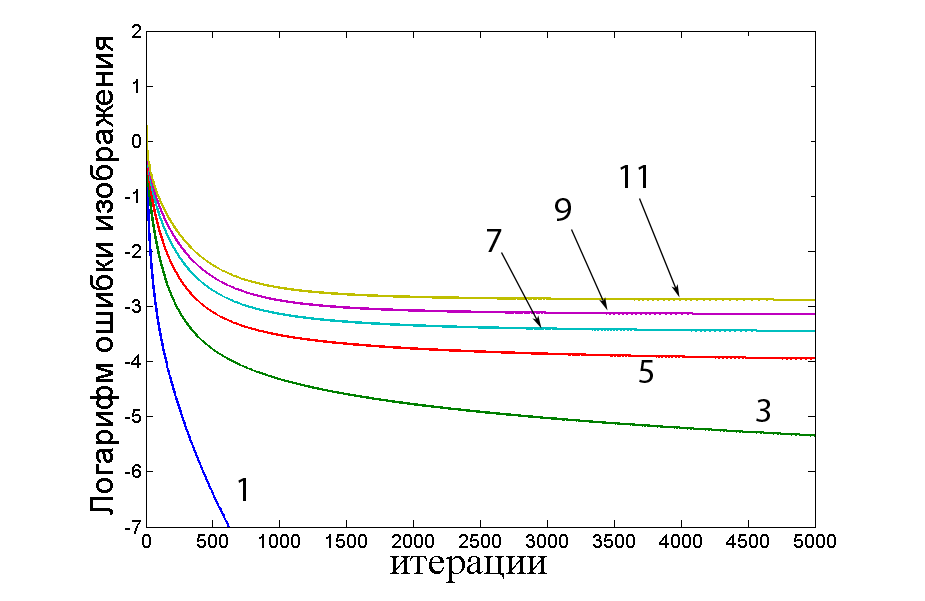
\includegraphics[width=0.50\textwidth]{Dissertation/images/part1_img/raw}
&
    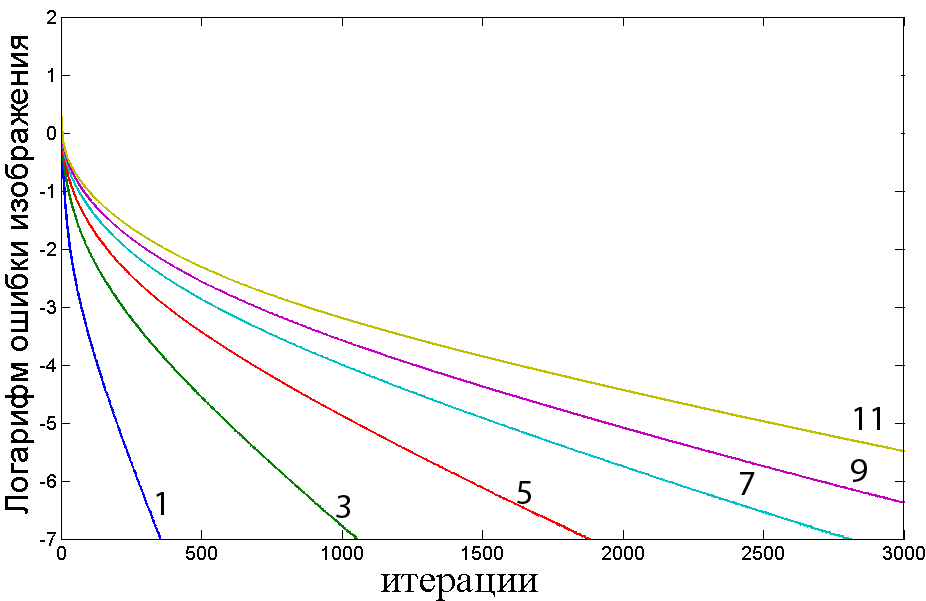
\includegraphics[width=0.50\textwidth]{Dissertation/images/part1_img/medk}
\\
   \small a) & \small b)
\end{tabular}
  \caption{Зависимость среднеквадратичной ошибки изображения от числа итераций.}
Номер графика соответствует степени разрежения. а --- Без регуляризации, б --- Медианный фильтр в качестве регуляризации.
\label{fig:conv_all}
\end{figure}

\vspace{2cm}

Еще одно преобразование, которое применяется к данным при переводе измеренных проекций из координат геометрии измерений $\rho, \varphi$ в координаты пространства БПХ, --- это учет изменения ширины БПХ-луча в зависимости от угла наклона, --- нормировка значений в строке по ширине и интенсивности:
\begin{enumerate}[label=\Roman*.]
	\item растяжение в $\frac 1 {\cos \alpha_i}$ раз
	\item растяжение в $\frac 1 {\cos \alpha_i}$ раз
	\item растяжение в $\frac 1 {\sin \alpha_i}$ раз
	\item растяжение в $\frac 1 {\sin \alpha_i}$ раз
\end{enumerate}

Чтобы повысить сходимость метода исследуются возможные регуляризации при применении метода FHT-SIRT.
Исследуются регуляризация с применением медианного, билатерального фильтров после каждой итерации, а так же регуляризация по Тихонову.
В последней части главы приводятся результаты восстановления с применением указанных видов регуляризации.
В частности, сравнение сходимости реконструкции без регуляризации и при использовании медианного фильтра приведено на рис. \ref{fig:conv_all} б).

\vspace{5mm}

В \underline{\textbf{третьей главе}} приведено описание предложенной модели формирования проекций при наличии в объекте сильнопоглощающих включений.
При прохождении через такие включения, например, металлический протез в зубе, большая часть зондирующего излучения поглощается.
В результате количество фотонов, достигающих детектора, недостаточно для активации его пикселя.
С таких пикселей считывается значение 0, хотя, на самом деле, можно лишь сказать, что значение, считанное с этих пикселей находится где-то в интервале $[0, \delta_{min})$, где $\delta_{min}$ --- минимальный порог срабатывания детектора, или уровень шума.
Восстановление без учета ошибок, содержащихся в синограмме, приведет к возникновению артефактов на восстановленном изображении (рис. \ref{im:quadprog}b,c). 

Для того, чтобы избежать появления этих артефактов, задачу восстановления в алгебраическом подходе можно модифицировать, вводя ограничения типа неравенства для пикселей, значение которых 0 (или $<  \delta_{min}$).
Для прологарифмированных значений, условие $I < \delta_{min}$ переходит в условие $f > \ln\frac{I_0}{\delta_{min}} = \delta$.
Тогда, с учетом перехода к логарифмам измеренной интенсивности, алгебраическая постановка задачи восстановления переходит в задачу условной оптимизации 

\begin{equation} \notag
  \label{eq:quadprog_ineq}
  \begin{cases}
  \Norm{P^{\textup{изм.}} - W(f)} \rightarrow \min\limits_f & w.r.t \\
  \sum_i f_{i} \omega_{ij} = P_j, & \mbox{если } P^{\textup{изм.}}_j < \delta \\
  \sum_i f_{i} \omega_{ij} > \delta, & \mbox{если } P^{\textup{изм.}}_j = \delta
  \end{cases}
\end{equation}

Так как функционал ошибки квадратичный, а ограничения - линейные, для решения этой минимизационной задачи эффективным будет применить метод квадратичного программирования.
При этом в формулировке оптимизационной задачи присутствует полная матрица преобразования Хафа $\omega_{ij}$.
Для размера восстанавливаемого изображения 256х256 и 180 проекционных углов при использовании типа данных float64 такая матрица будет занимать порядка 32Гб.
Общая формула для расчета размера матрицы это $\sqrt{2} * n * n_\varphi \times n * n$.
При этом ненулевые значения для каждого столбца находятся только в $\approx n$ ячейках, делая возможным использование инструментария для работы с разреженными матрициы.

Результаты востановления методом квадратичного программирования представлены на рис. \ref{im:quadprog}.
Результаты представлены на небольшом фантоме размера 10х10 пикселей и 35 проекционных углов.

\begin{figure}
  \centering
  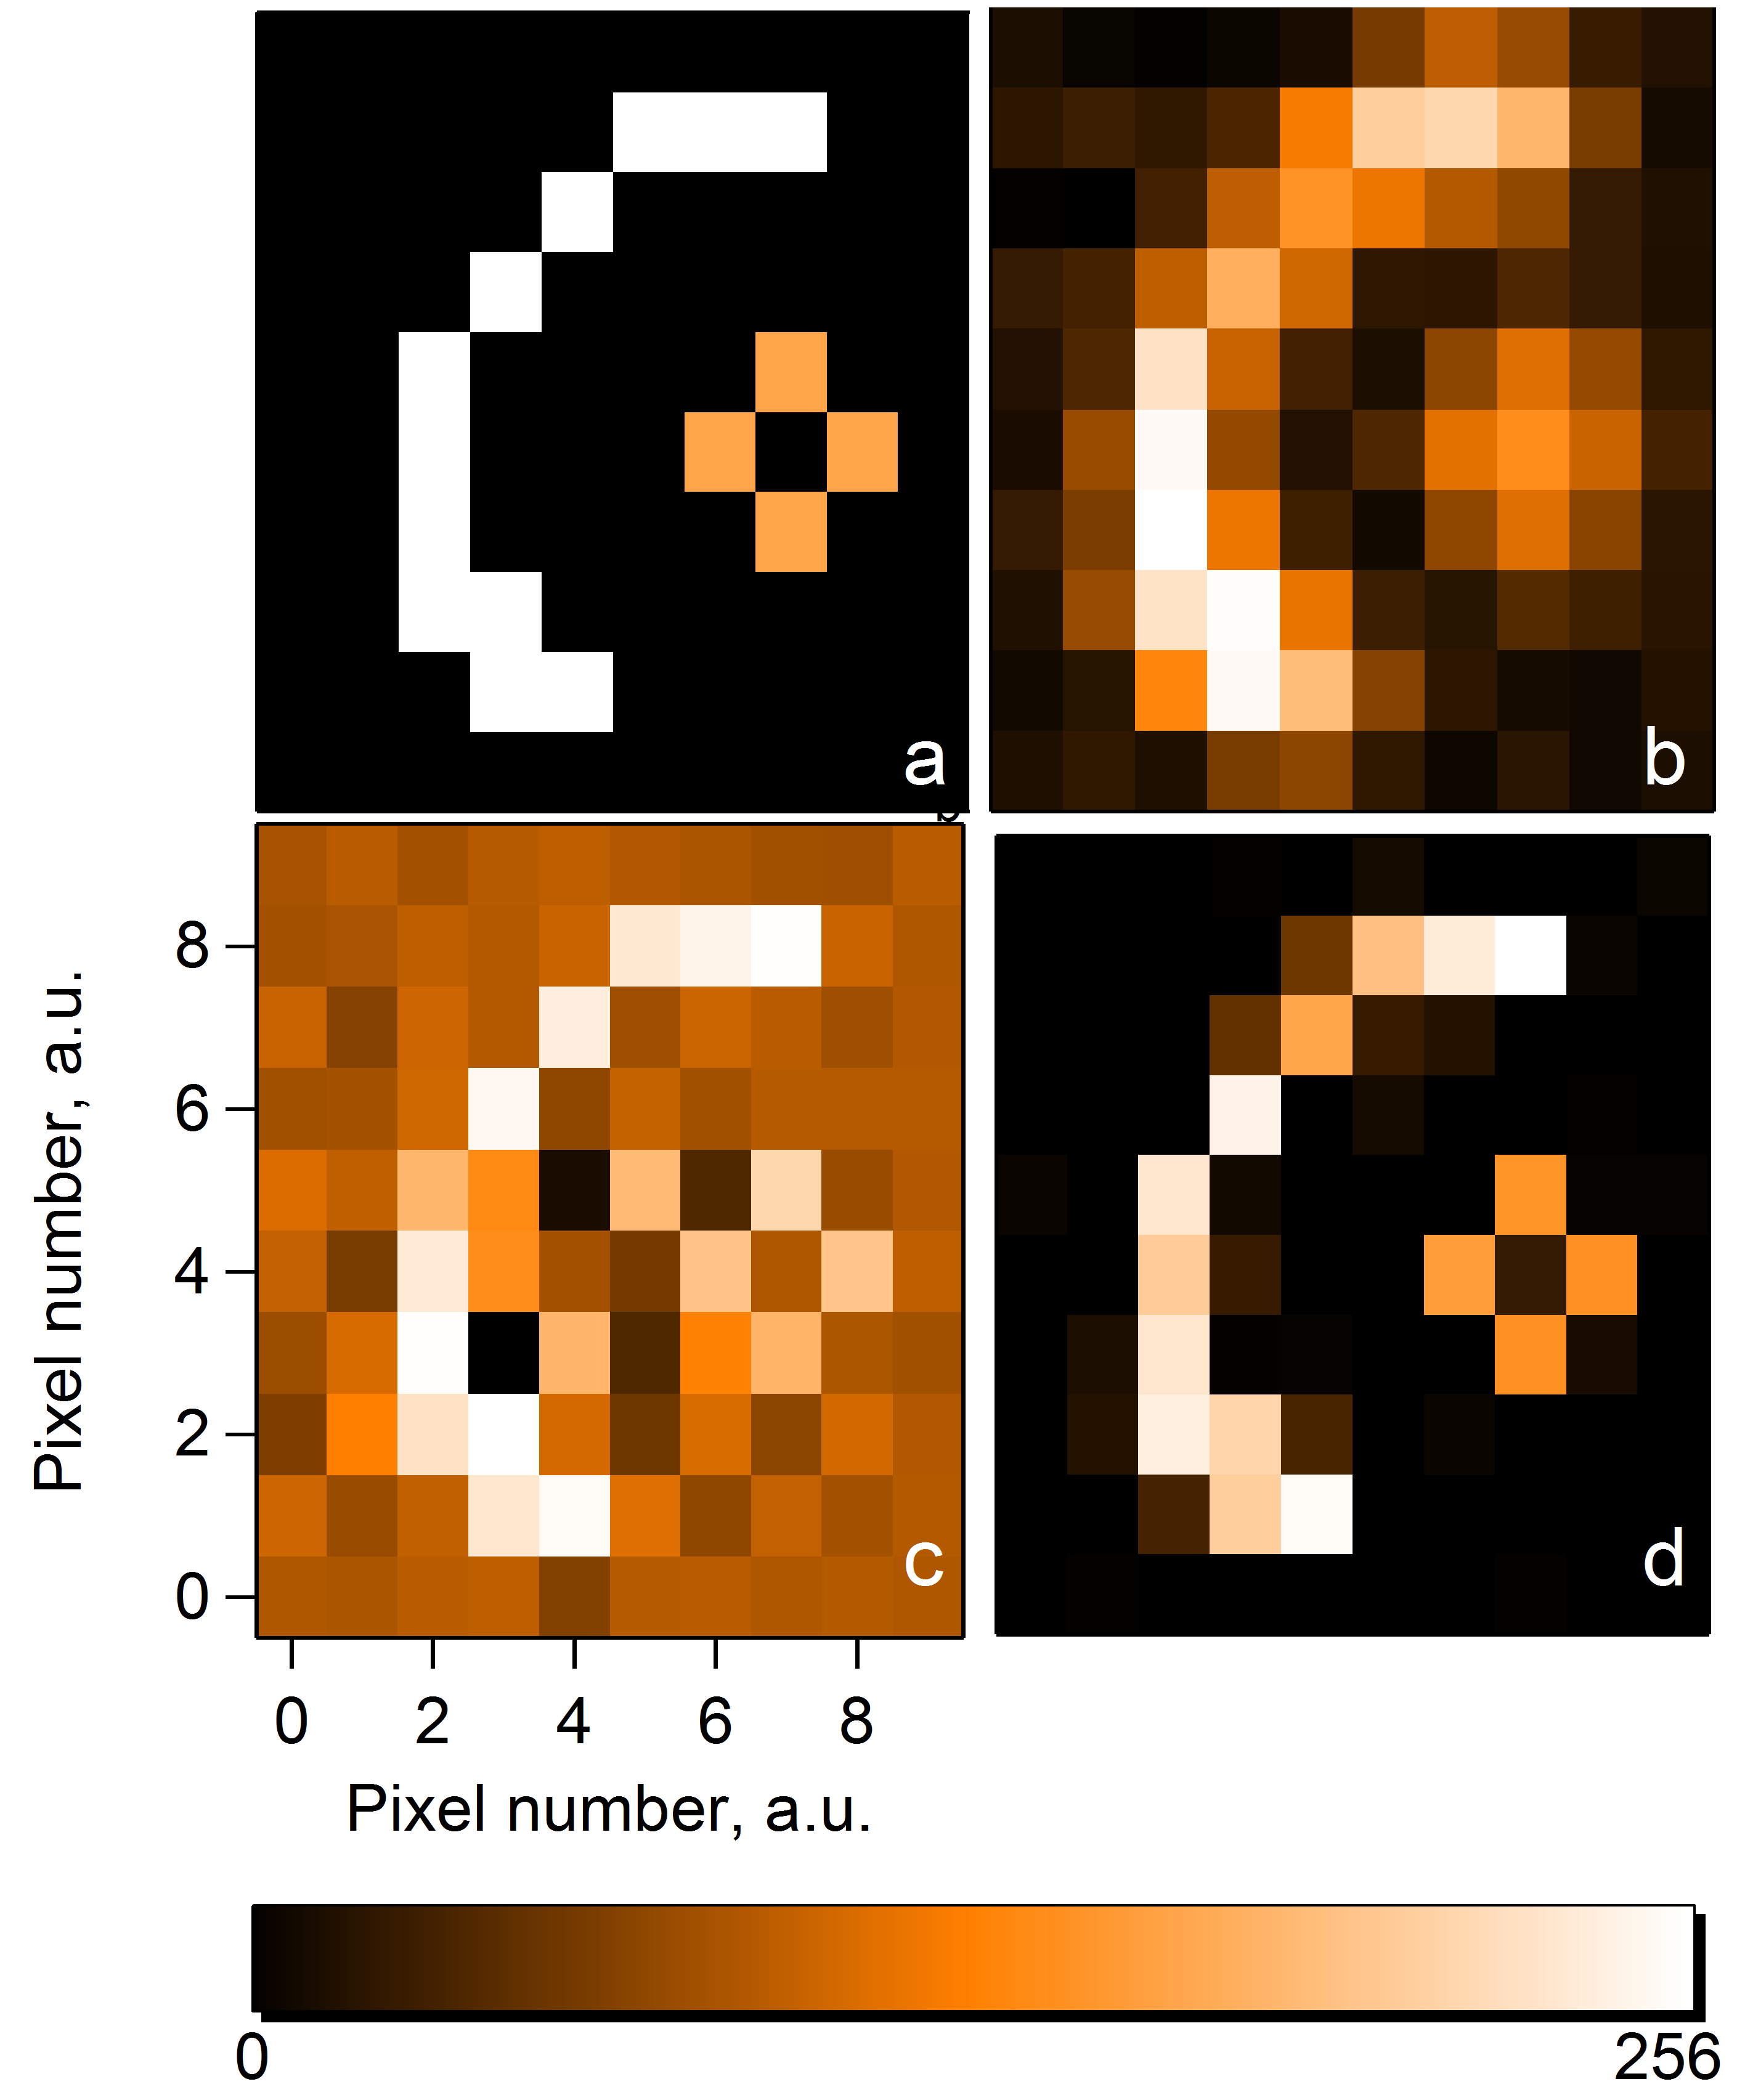
\includegraphics[width=0.8\textwidth]{Dissertation/images/part2_img/quadprog}
  \caption{Слева-направо сверху-вниз: a) - фантом, использованный для расчета лучевых сумм. b)- результат восстановления методом FBP. c) - результат восстановления методом квадратичного программирования без ограничений-неравенств. d) - результат восстановления методом квадратичного программированиея с учетом ограничений-неравенств (предложенный метод)}
  \label{im:quadprog}
\end{figure}

Использование жестких ограничений не всегда стабильно отностильно наличия шумов в данных.
Этот подход так же требует работы с матрицей проекции, которая даже в разреженном виде требует больших вычислительных ресурсов.
Этого можно избежать, если заменить уравнения ограничений задачи оптимизации на аддитивные квадратичные регуляризирующие штрафы, выражающие эти ограничения.
Такой подход называется методом мягких ограничений.
В контексте решаемой задачи и ее ограничений, предлагается ввести квадратичные штрафы за нарушение выхода за границы порога $\delta$.
Если ввести диагональные матрицы-индикаторы нарушения ограничений, $J_{ii} = \left\{1, \mbox{если} \left(\sum f_{i} \omega_{ij} > \delta \right), \mbox{иначе } 0\right\}$, и $K = E - J$, то задача минимизации с мягкими ограничениями будет выглядеть как

\begin{equation} \notag
  \label{eq:soft-ineq}
  ||K(Wf - P^{\textup{изм}})||^2 + \alpha ||J(Wf - \Delta)||^2 \to \min\limits_f,
\end{equation}

В работе проводится исследования метода мягких ограничений с использованием данных лабораторных измерений.
Измерения проводились на прототипе программно-аппаратного томографического комплекса созданного и функционирующего в лаборатории рефлектометрии и малоуглового рассеяния ФНИЦ ``Кристаллография и фотоника'' РАН.
Восстановления фантомов, а так же реального образца, можно наблюдать на рисунках.
В работе производится сравнение восстановления методами мягких ограничений и метода квадратичного программирования.

\begin{figure}
  \centering
  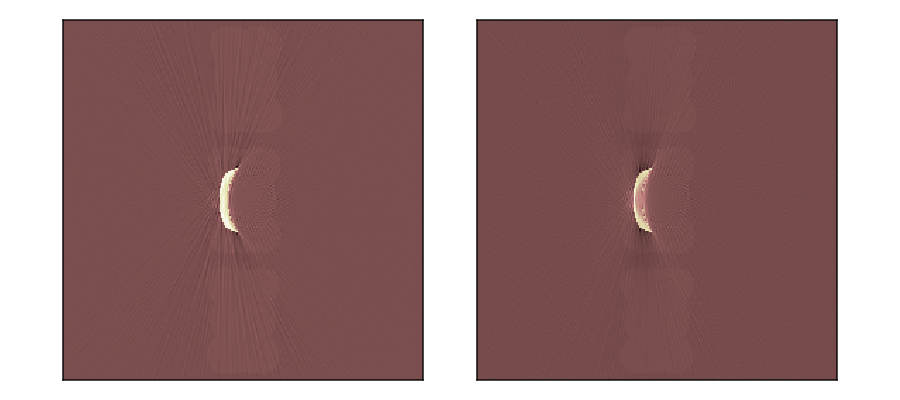
\includegraphics[width=0.9\textwidth]{Dissertation/images/part2_img/sample}
  \caption{Реконструкции методом мягких ограничений.}
  \label{fig:sample}
\end{figure}

\vspace{10mm}

На рис. \ref{fig:sample} представлены результаты реконструкции фантома, моделирующего золотое (Au) включение в зубе (Ca).
Результаты восстановления методом мягких ограничений (слева) и методом, в которых данные выше порога просто игнорируются (справа), 200 итераций алгебраического метода, коэффициент регуляризациии --- 30.

\begin{figure}
\centering
\begin{tabular}{@{}c@{}c}
    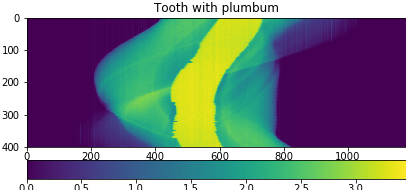
\includegraphics[width=0.50\textwidth]{Dissertation/images/part2_img/tooth_sino}
&
    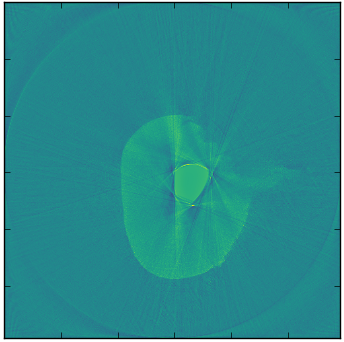
\includegraphics[width=0.50\textwidth]{Dissertation/images/part2_img/soft_ineq_pb_tooth}
\\
   \small a) & \small b)
\end{tabular}
  \caption{a --- Синограмма молочного зуба с включением из свинца. б --- результат восстановления методом мягких ограничений}
\label{fig:tooth_sino_rec}
\end{figure}

В качестве реального образца была взята синограмма зуба со свинцовым включением.
В качестве порога было выбрано значение 2.9, соответствующее последнему пику интенсивности на гистограмме синограммы.
Обоснование выбора этого значения проиллюстрировано на гистограмме на риc. \ref{fig:pb_hist}.


\begin{figure}
	\centering
	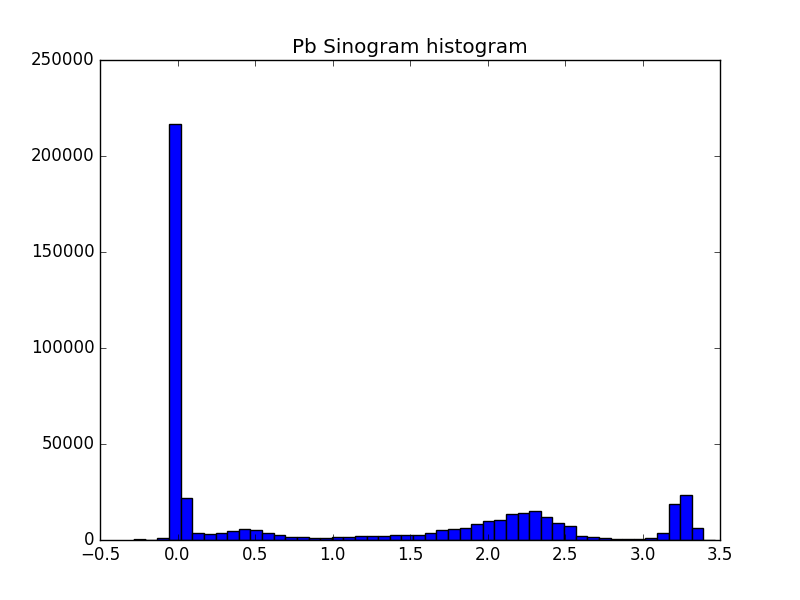
\includegraphics[width=0.9\textwidth]{Dissertation/images/part2_img/pb_hist}
	\caption{Распределение интенсивностей синограммы}
	\label{fig:pb_hist}
\end{figure}



\vspace{5mm}

В \underline{\textbf{четвертой главе}} описан предложенный подход для восстановления томографических измерений при зондировании полихоматическим илучением, основанный на использовании алгебраического метода реконструкции.
В большом количестве экспериментальных схем спектр источника является полихроматическим, то есть энергия источника имеет нетривиальный несингулярный спектр.
Использование монохроматора, с одной стороны, позволяет понизить сложность задачи реконструкции, сведя решение к монохроматическому случаю, но это увеличивает время получения набора томографических проекций, с другой стороны.
Это делает метод неприменимым для практической медицины и промашленной интроскопии.
Свойства поглощения материала меняются в зависимости от частоты зондирующего излучения.
В результате, реальная измеренная детектором интенсивность рентгеновского излучения не соответствует модели, используемой в традиционных подходах к восстановлению.
Это значит, что заложенные в алгоритме реконструкции модели прямой и обратной проекции либо будут неспособны обеспечить сходимость оптимизационной процедуры, либо сойдутся к ложному минимуму, не являющемуся в реальности решением физической задачи.
В обоих случаях восстановление традиционными алгоритмами синограммы, снятой при зондировании немонохроматическим излучением, повлечет появление артефактов на восстановленном изображении.

В данной главе рассматривается метод, позволяющий учесть спектральные особенности взаимодействия материалов объекта с излучением.
При этом предлагается перейти от восстановления распределения линейного коэффициента ослабления излучения к восстановлению пространственного распределения концентраций элементов $c_k(x,y)$, массовые коэффициенты ослабления которых затабулированы:

\begin{equation} \notag
  \label{eq:white_fp_final}
  I(c)_j = \int_0^{+\infty} {d\lambda \left\{
    I_0(\lambda) \exp{\left(
      -\sum_{k=1}^K {\rho \kappa_k(\lambda) (W c_k)_j} 
      \right)}
  \right\}}
\end{equation}

,здесь за $\kappa_k(\lambda)$ обозначен массовый коэффициент поглощения вещества $k$ на длине волны $\lambda$, а $I_0(\lambda)$ --- спектр источника, $\rho$ --- линейный размер пикселя, индекс $j$ обозначает номер пикселя на изображении измеренных проекций.
Следуя алгебраическому подходу, реконструкция проводится с помощью градиентного спуска оптимизации квадратичной функции потерь 
$
Q(c) = \frac {\left(I(c) - t\right)^2} {S}
$
, где $t$ --- измеренные интенсивности прошедшего через объект излучения, 
$S = \int_0^{+\infty} { I_0(\lambda) d\lambda}$
 --- суммарная интенсивность зондирующего излучения.

Общий вид итерации восстановления будет иметь вид

\begin{equation} \notag
\label{eq:part3_whitegrad}
  \nabla_k \ Q = 2W^\intercal R_k \text{, где } R_{kj} = \frac {(I(c) - t)_j} {S} \mu_{kj}
\end{equation}
, а формулы для вычисления весов невязок по каждому элементу приведены ниже:
\begin{equation} \notag
  \label{eq:weights}
  \mu_{k} = \int_0^{+\infty} {d\lambda \left\{
    -\rho \kappa_k(\lambda) 
    I_0(\lambda)
    \exp{\left(
      -\sum_{s=1}^K {\rho \kappa_s(\lambda) (W c_s)} 
         \right)}
    \right\}}
\end{equation}

В указанной итерационной схеме отсутсвует пространственные различия в формулах обновления концентраций разных элементов. 
Поэтому необходимо вводить дополнительную регуляризацию.
Предлагаемое решение состоит в том, чтобы запретить находиться в одной пространственной ячейке одновременно разным материалам $c_{k_1} \odot c_{k_2} = 0, \mbox{если } k_1 \neq k_2$, что при применении метода мягких ограничений выглядит как аддитивный регуляризующий член 
\begin{equation} \notag
	\sum_{k_1 != k_2} {||c_{k_1} \odot c_{k_2}||^2}
\end{equation}

Здесь за $c_{k_1} \odot c_{k_2}$ обозначена поэлементная операция умножения массивов.
На рисунке \ref{fig:whiteres} представлены результаты восстановления для фантома с использованием и без использования регуляризации.
На верхнем ряду представлены распределения концентраций каждого элемента в первых двух столбцах, а в третьем - их отношение.
Наблюдать отношение концентраций разных элементов полезно для контроля пространственного разделения их характеристик.
В случае, если оптимизация вырождается по координате элементов, третий столбец будет равномерно одинакового значения.
Снизу представлены аналогично преобразования Хафа для концентраций элементов и их отношения в третьем столбце.

\begin{figure}
\label{fig:whiteres}
\centering
\begin{tabular}{@{}c@{}c}
  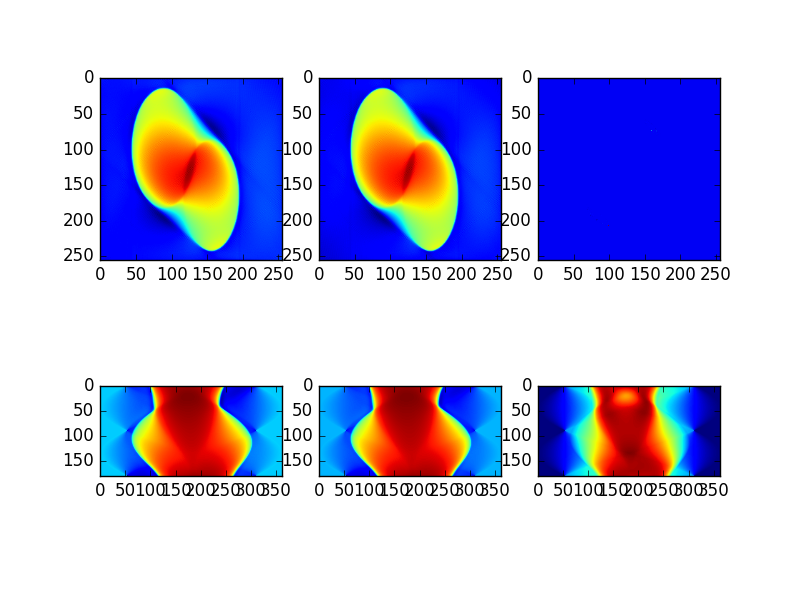
\includegraphics[width=0.5\textwidth]{Dissertation/images/part3_img/no_reg_iteration_25} &
  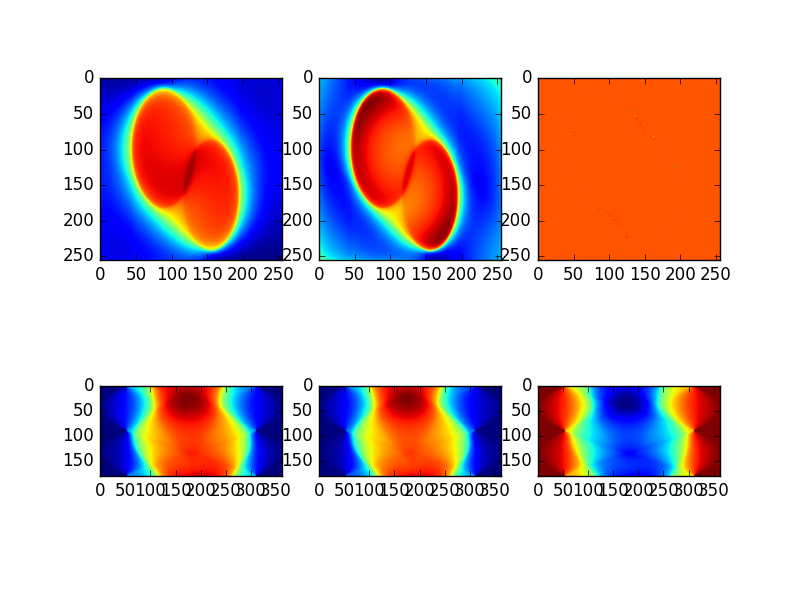
\includegraphics[width=0.5\textwidth]{Dissertation/images/part3_img/mul_reg_iteration_150}
  \\
  а) &
  б) \\
\end{tabular}
\caption{Восстановление с помощью МВН. а) без регуляризации. б) мультипликативная регуляризация}
\vspace{5mm}
\end{figure}


Как видно из рисунков, мультипликативная регуляризация позволяет пространственно разделить концентрации различных элементов.

В \underline{\textbf{заключении}} приведены основные результаты работы, которые заключаются в следующем:
%% Согласно ГОСТ Р 7.0.11-2011:
%% 5.3.3 В заключении диссертации излагают итоги выполненного исследования, рекомендации, перспективы дальнейшей разработки темы.
%% 9.2.3 В заключении автореферата диссертации излагают итоги данного исследования, рекомендации и перспективы дальнейшей разработки темы.
\begin{enumerate}
  \item Получено аналитическое выражение для операции транспонированного быстрого преобразования Хафа. Доказана теорема о симметричности четверти БПХ, отвечающей одной группе ориентаций лучей. Получен метод вычислительно эффективного вычисления транспонированного преобразования.
  \item Построен вычислительно эффективный алгебраический метод восстановления измерений компьютерной томографии на основе БПХ. Произведена адаптация метода для работы с данными реальных измерений. Изучены свойства пространства БПХ, влияние различной регуляризации на процесс восстановления.
  \item Построен метод восстановления рентгеновской томографии методом квадратичного программирования для объектов, содержащих сильнопоглощающие включения. На реальных экспериментальных измерениях проведено исследование метода мягких ограничений \todo{и сравнение с методом квадратичного программирования}
  \item Построен алгебраический алгоритм восстановления томографии в задаче зондирования полихроматическим излучением, основанный на вычиследнии взвешанных невязок по каждому из элементов, входящих в состав исследуемого образца. Предложены варианты регуляризации для востановления в полихроматической моде. \todo{описать, какой получен результат}
\end{enumerate}


\begin{comment}
%\newpage
При использовании пакета \verb!biblatex! список публикаций автора по теме
диссертации формируется в разделе <<\publications>>\ файла
\verb!../common/characteristic.tex!  при помощи команды \verb!\nocite! 
\end{comment}

\newpage
\ifdefmacro{\microtypesetup}{\microtypesetup{protrusion=false}}{} % не рекомендуется применять пакет микротипографики к автоматически генерируемому списку литературы
\ifnumequal{\value{bibliosel}}{0}{% Встроенная реализация с загрузкой файла через движок bibtex8
  \renewcommand{\bibname}{\large \authorbibtitle}
  \nocite{*}
  \insertbiblioauthor           % Подключаем Bib-базы
  %\insertbiblioother   % !!! bibtex не умеет работать с несколькими библиографиями !!!
}{% Реализация пакетом biblatex через движок biber
  \ifnumgreater{\value{usefootcite}}{0}{
%  \nocite{*} % Невидимая цитата всех работ, позволит вывести все работы автора
  \insertbiblioauthorcited      % Вывод процитированных в автореферате работ автора
  }{
  \insertbiblioauthor           % Вывод всех работ автора
%  \insertbiblioauthorgrouped    % Вывод всех работ автора, сгруппированных по источникам
%  \insertbiblioauthorimportant  % Вывод наиболее значимых работ автора (определяется в файле characteristic во второй section)
  % \insertbiblioother            % Вывод списка литературы, на которую ссылались в тексте автореферата
  }
}
\ifdefmacro{\microtypesetup}{\microtypesetup{protrusion=true}}{}

      % Содержание автореферата

%%% Выходные сведения типографии
\newpage\thispagestyle{empty}

\vspace*{0pt plus1fill}

\small
\begin{center}
    \textit{\thesisAuthor}
    \par\medskip
    
    \thesisTitle
    \par\medskip
    
    Автореф. дис. на соискание ученой степени \thesisDegreeShort
    \par\bigskip
    
    Подписано в печать \blank[\widthof{999}].\blank[\widthof{999}].\blank[\widthof{99999}].
    Заказ № \blank[\widthof{999999999999}]
    
    Формат 60\(\times\)90/16. Усл. печ. л. 1. Тираж 100 экз.
    %Это не совсем формат А5, но наиболее близкий, подробнее: http://ru.wikipedia.org/w/index.php?oldid=78976454
    
    Типография \blank[0.5\linewidth]
\end{center}
\cleardoublepage

\end{document}